\documentclass[a4paper,man,natbib,floatsintext,mask]{apa6}
\usepackage[utf8]{inputenc}

\usepackage{rotating}

\usepackage{subcaption}

\usepackage{todonotes}
\usepackage{tikz-qtree}
\usepackage{threeparttable}

\title{Detecting and analyzing news events}
\shorttitle{Detecting and analyzing news events}

\author{Damian Trilling \& Marieke van Hoof}

\affiliation{University of Amsterdam}

\abstract{When comparing media coverage or analyzing which content people are exposed to, researchers usually do not conduct their analyses on the level of an individual article, but choose a level of abstraction, such as topics or issues. In this paper, we develop a theoretical argument for introducing the ``news event'' as a level of analysis. Based on this, we discuss several computational approaches to empirically detect such news events in large corpora of news coverage in an unsupervised manner. In particular, we compare approaches based on traditional tf$\cdot$idf based cosine similarities with approaches that rely on word embeddings, such as the softcosine measure. We show that both methods, combined with a network clustering algorithm, are suitable to detect news events. Finally, we apply this method in a case study of 45k news articles from different outlets, in which we show that different news outlets have distinct profiles in the events they cover.}

\keywords{news events, text mining, text analysis, unsupervised, network clustering}

\begin{document}
\maketitle

\section{Introduction}
Modern democratic societies are unthinkable without journalism. %While journalism is undergoing significant changes due to a changing media environment as well as social and technical developments, its fundamental tasks remain unchanged. One of these tasks is the \emph{dissemination of information} \citep[e.g.,][]{Beam2009}.
One of the tasks of journalism is the \emph{dissemination of information} \citep[e.g.,][]{Beam2009}.
This implies that in a well-functioning media system, there will be a comparatively large overlap in terms of events that are covered by different outlets.
In particular, large parts of journalism involve \emph{routine reporting}, which ensures that information about routine events (parliamentary debates, elections; but also figures about the economy, cultural events, sports, \ldots) are disseminated to a wide audience.
News value research has investigated which news events are usually considered newsworthy, and suggests that these news values are largely shared by journalists across contexts \citep[e.g.,][]{Eilders2006,Harcup2016}.

Even exclusive stories, based on ideas or information only available to one outlet, are ultimately reported on by other outlets as well.
Take the example of \emph{investigative reporting} \citep[see, e.g.,][]{deburgh2008}, which ensures that scandals are discovered and that public officials can be hold accountable.
Investigative reporting requires extensive research, which makes it costly both in terms of time and resources -- but at the same time, it gives large recognition to the journalists discovering the scandal.
But once one outlet published its information, others will jump on it as well, either by paraphrasing the article from the original outlet or by writing follow-up stories.
Take the Watergate scandal: While all credits for uncovering it have to go to Bob Woodward and Carl Bernstein of The Washington Post, its immense political significance made all other media report on it as well after the story broke -- which, in fact, is necessary to make investigative reporting effective and exert political pressure.
We see that, both in the cases of rather ``boring'' routine reporting and major scoops, one \emph{news event} is often covered by multiple articles in multiple outlets, to a potentially very different extent and in very different styles (e.g., choosing different words).
This makes the task to identify articles covering the same event a challenging one.
Yet, in order to systematically compare the coverage of an event between outlets, we need to do so.

Shifting our focus from news production to news consumption, we face the same challenge:
Tracking data or digital trace data may give us very fine-grained information on which specific articles someone has read, but to compare consumption patterns or study exposure effects, we somehow have to group related articles.
In this work, we argue that for both theoretical and methodological reasons, we need to do so on the level of what we refer to as \emph{news events}.
Many theories of democracy assume a citizenry that has a more or less shared awareness of relevant events happening \citep{Ferree2002,Stromback2005}.
 This is even true for models that acknowledge that most citizens are actually rather uninvolved in politics. Here, ``rather than  try  to  follow  everything,  the  monitorial  citizen  scans  the  environment  for  \emph{events}  that  require  responses'' \citep[p.~118; emphasis ours]{Zaller2003}. Yet, most research has investigated the existence of a ``common core of issues''  \citep[e.g.,][]{Chaffee2001,Geiss2018b,Moeller2016}, whereas we argue that it might actually be at least as informative to investigate a ``common core of events'' that people are aware of. In fact, in line with the monitorial citizen model, it has been shown that in periods of high political activity, the events that citizens read about are more closely aligned with the events journalists deem most important \citep{boczkowski2013}. 

News events, in our understanding, are more specific than a topic or an issue, but less specific than an individual article (or tv news item, video, etc.). For instance, a news website can choose to devote zero, one, or more articles to one event; and in fact, that's often done. A short breaking-news article, might be followed up with a larger, more extensive piece, an update, an opinion piece, and/or an interview. A competitor's website might make different choices, while still covering the same event.

To understand and analyze the role of the media in a given democratic society, we therefore need to solve a central problem: \emph{How can we identify and distinguish news events in media coverage?}

In this paper, we offer a conceptualization of \emph{news events} and a method to detect such news events. For the sake of simplicity, we will assume written news (on news sites, in newspapers, etc.) and will refer to the individual news item as an ``article''. Our argumentation and theoretical definition can be extended to audiovisual news, but the specific method we present is focused on textual content.

We then apply our method to a case study, in which we identify news events in a dataset of 45K articles from three Dutch news outlets spanning a period  of half a year.
In particular, we investigate in how far the coverage of events overlaps between outlets, and the amount of coverage that different events generate.
This allows us to assess in how far coverage can be seen as uniform (at least in terms of \emph{what} is covered, not \emph{how} it is covered) or fragmented.




\section{Theoretical background and related work}

In order to develop our approach to the study of news events, we proceed in three steps. 
First, to show why it is important to study news events, we discuss areas of communication research to which our proposed method to identify and analyse news events may be particular relevant: agenda setting research, media hype research, and audience research.
Then, we develop a working definition of news events.
Finally, we review different methods that may be used to automatically identify news events.
After that, we will develop our methodological approach and apply it to a first case study.


\subsection{Why do we need to study news events?}
\subsubsection{News events and agenda setting}
The temporal dynamics of news event coverage is of key interest to agenda setting researchers, in particular to those studying inter-media agenda setting.
We know from agenda setting research that once an exclusive story has been published by a powerful outlet, others are going to take it over.
For instance, \citet[p.~12]{mccombs2009} write: ``The New York Times frequently plays the role as intermedia agenda-setter because appearance on the front page of the Times can legitimize a topic as newsworthy''.
Interestingly, already in \citeyear{Larsen1954}, \cite{Larsen1954} studied empirically the ``diffusion of a news event'', in their case the question via which media and when members of different communities heard about the death of a senator. Developing an automated approach to identify news events will allow us to conduct such and similar studies on a much larger scale.

However, we need to add a cautionary note here. The ``old'' media system was characterized by typically one newspaper edition per day\footnote{Although at the beginning of the 19\textsuperscript{th} century, some newspapers published multiple editions per day.}. Even though causal inferences from content analysis data are always problematic, this gave agenda-setting studies the opportunity to build on the assumption that a time lag in publication could be interpreted as an agenda-setting influence.

But even though there are some cases where timestamps have been successfully used to demonstrate \textit{online} intermedia agenda-setting processes \citep{Haim2018a}, the fact that contemporary online outlets may publish on the same topic within minutes or hours makes it much harder to draw such inferences.
Next to that, while many agenda-setting studies relied on rather broad categories  \citep[see, e.g.][]{Baumgartner2006}, recent societal issues may not fit into these.
For instance, studies on the agenda-setting power of so-called ``fake news'' highlighted that a more fine-grained approach is needed, in which coverage of one specific event --- be it a real one or a fabricated one --- can be traced across outlets \citep{VanHoof2019,Vargo2018}.


\subsubsection{News events and media hypes}
The ``event'' is also a central term in Vasterman's (\citeyear{Vasterman2005}) work on news waves and media hypes. Building on \cite{Kepplinger1995}, Vasterman identifies so-called ``key events'' that trigger media coverage. He argues that in what he calls a media-hype, media are then ``making the news instead of reporting events by: reporting comparable incidents and linking them to the key event; reporting thematically related news such as features, analyses and opinions'' (p.~516).
He distinguishes between genuine events (``like violent incidents or court convictions'', p.~528) that are happening in the real world, independently of news coverage and other events, such as ``an interview, a speech, an official warning (regarding health risks) or, as often happens in scandals, a startling disclosure by investigative reporter'' (p.~514). Importantly, key events can be of either category.

Very much like what is the key objective of our paper, researchers working on news waves and media hypes are interested in identifying articles related to one event. However, they typically define the event in advance (see, e.g, \cite{Hellsten2015} for a typical example), while we assume that events are not known a priori.
As we will elaborate on below, our conceptualization of a ``news event'' differs slightly from the terminology used in media hype research. In our conceptualization, an interview that follows up upon a news story on, say, a violent incident, would be considered as belonging to the same event, whereas \cite{Vasterman2005} would see both articles as belonging to the same ``news wave'', but the interview being a separate event.


\subsubsection{News events and audience research}
Finally, the study of news events becomes increasingly relevant for audience research.
Audience research is facing large transformations, in which tracking data and digital trace data become more and more important. 
This abundance of data poses new challenges in how to abstract and aggregate.
For instance, if we have data on the browsing histories of respondents \citep[for a data collection tool, see][]{Menchen-Trevino2016}, we need to settle on a level of analysis on which the abundance of URLs that people visited can be aggregated.
For instance, one could consider the domain level and investigate in how far the outlets people regularly visit overlap \citep[e.g.,][]{Mukerjee2017}.
While this can be informative to study, for instance, whether the audiences of extremist and mainstream media overlap, it does not help us to address another issue that is of core interest from a theoretical point of view:
answering the question whether there is a fragmentation of the public sphere \citep[see, e.g.,][]{Marcinkowski2008} such that some groups of people are not aware of the same events happening in society as others.
Therefore, audience research that uses digital trace or tracking data needs to develop methods that allow to group articles that are covering the same event \citep[see also][]{Trillingnetwork}.



\subsection{How can we define news events?}
Having identified the significance of the study of news events to multiple areas in communication science, we proceed to developing a working definition of a news event.
There is an infinite number of things happening in the world, and what ``becomes news'' is not only determined by objectively measurable characteristics, even though news value research offers some characteristics that may increase the likelihood of something being considered a newsworthy event by journalists \citep[e.g.,][]{Eilders2006,Harcup2016}.
However, this does not help us much to define what \emph{the event} that is covered actually is.  
Even seemingly simple characteristics of an event, such as its scope, its beginning and end, are hard to define. For instance, a public clash between two politicians of the same party probably is a newsworthy event. But is the speech that the first politician gives one event and the reaction of the second another one? Or is neither, and is the occasion where it happened (let's say, a party congress) the event?
As this example illustrates, the decision how the stream of what's happening is chunked into meaningful ``stories'' is largely contingent, and thus, news can be seen as ``a socially determined construction of reality'' \citep[p.~428]{Staab1990}.

Consequently, any attempt to determine the one-and-only event classification of what happens on a given day is doomed to fail. On the other hand, unless one denies the existence of any physical reality, one must acknowledge the existence of events that spark media attention: the final match of a world championship, a sudden invasion of one country by another, an earthquake. 
If we want to determine, for instance, in how far news outlets publish about the same news event as others, we are not interested in an individual news article, but in all articles that cover such a \emph{news event}. We therefore preliminary define news events as follows: 

\begin{quote}
News events are specific events that lead to news coverage, such as a specific debate on a specific day in a specific parliament, a specific accident, or a specific football match. They can be covered by one or more articles in one or more outlets, but relate to one specific and identifiable event and are thus much more fine-grained than news topics, issues, or news categories.
\end{quote}
Figure~\ref{fig:model} offers a graphical illustration of an example of this definition. 


\begin{sidewaysfigure}[ht!]
\tikzset{edge from parent/.style=
{draw, edge from parent path={(\tikzparentnode.south)
-- +(0,-8pt)
-| (\tikzchildnode)}},
blank/.style={draw=none}}
\begin{tikzpicture}
\matrix
{
\node{\Tree
    [.\textbf{ }  \edge[blank]; 
    [.\textbf{Topic}  \edge[blank];
    [.\textbf{News\ event} \edge[blank]; 
    [.\textbf{Article} ]]]]};
&
\node{\Tree 
 [.All\ news 
    [.Politics 
        [.Parliamentary\ debate\ on\ X  1 2 3 ] 
        [.Local\ election\ result\ in\ X  1 ] 
        ]
    [.Accidents,\ disasters,\ ... 
        [.Accident\ on\ highway\ Y  1 2 3 4 5 6 ] ]
    [.Sports
        [.Club\ A\ defeats\ club\ B 1 2 3 ] ]
        ]}; \\
};        
\end{tikzpicture}
\caption{News events can be covered by one or more articles in one or more outlets, but relate to one specific and identifiable event and are thus much more fine-grained than news topics or news categories. \label{fig:model}}
\end{sidewaysfigure}


% dirty hack to get the conceptual figure at least before the methods start
\clearpage


Our conceptualization of what an event can be is notably broader than in some other fields. For instance, the GDELT Project (\url{https://www.gdeltproject.org/}) defines an event as ``capturing two actors and the action performed by Actor1 upon Actor2'' \citep[p.~41]{GDELT}, and furthermore is focused on international politics\footnote{Nevertheless, GDELT is also used within the discipline of communication science \citep[see][]{hopp2019}.}. GDELT extracts event data from media coverage, which seems similar to our approach -- but it is a fundamentally different one. While we are in principle interested in any event, and while these events are a priori completely unknown and unrestricted, GDELT aims at extracting events such as  ``Country A attacks Country B''. In this sense, the events in the GDELT database would fit our concept of a news event, but the reverse is not necessarily true.

Instead, our conceptualization of news events is more similar to the notion of news story chains by \cite{Nicholls2018}, who ``define news `story chains' as events or single issues which receive repeated coverage in the news media through a series of initial articles and followup pieces'' (p.~44). The differences are, in fact, subtle; nevertheless, they result in a different analytical and interpretative lens. First, the notion of a chain evokes the image of a strict (temporal) order. However, especially when analyzing coverage of the same events across multiple outlets, it may not always be meaningful to say ``who was first'', and links between articles may be more complex: If two outlets A and B publish two articles A1 and B1 about the same event on day 1, B publishes a follow-up B2 on day 2 (but A does not), and both A and B publish articles A3 and B3 on day 3: how would the chain look like? What is the predecessor of A3? Is it B2 or A1? And is A1 or B1 the ``initial article''? Depending on the specific research question, either the temporal notion of a story chain or our more general notion of a news event may be more useful. 
Second, \cite{Nicholls2018} are interested in ``repeated coverage'' only, while here again our scope is wider: a standalone article that covers one event covered by no one else is within the scope of our definition of a news event, but not within the scope of the definition of a news story chain. Again, which is more useful depends on the research question.

Still, the notion of a news story chain and a news event have more commonalities than differences. Most notably, they introduce a more fine-grained level of analysis than the often-used topic: ``News stories are conceptually distinct from news `topics,' which we define as thematic news areas which also receive repeated coverage but which naturally encompass multiple events, and whose time span is much longer (indeed many news topics are essentially permanently recurring features of news coverage)'' \citep[p.~44]{Nicholls2018}.
Figure~\ref{fig:model} illustrates how the analytical level of a news event is situated between a topic and an individual article. 
Typically, given a large-enough corpus, we would assume that one news event often triggers multiple articles (especially given that the bulk of events will be covered by multiple outlets). For instance, \cite{Buhl2016} grouped 1,919 online news reports into 131 events, and \cite{Nicholls2018} automatically identify 5,753 ``story chains'' in 39,558 articles.

It is an interesting question whether the opposite is possible as well. One could conceive of a situation in which one article covers multiple events; for instance an analytical background piece in the weekend edition of a newspaper, reflecting on several events happening that week; or a longer feature story in a magazine. How often this happens is an empirical question.\footnote{In practice, we expect it to be very challenging to detect multiple events within one article when using document-level comparisons. An article discussing two events will have only medium-level similarities with each article that discusses one event exclusively.}
For now, we will focus on the typical case, in which an article reports on one event only.

A second consideration is how events are grouped into topics or issues. Again, we can ask whether an event can belong to multiple issues. An example of that approach would be agenda-setting studies like the Comparative Agendas Project \citep{Baumgartner2006}. Topics or issues are often coded in a hierarchical manner, with broader topics having sub-topics; while at the same time allowing one article being assigned multiple topics and/or subtopics. On the other hand, ultimately, many analyses in such studies are focusing on the analysis of the ``main topic'' of articles, substantiating the argument that it is possible to assign a news event to one topic.

A third consideration is how news events are related to each other. One possible approach is to simply treat them as unrelated, which may be suitable when interested, for instance, in the question how many different events are covered by which outlets. Another possibility would be to threat them as related via their parents in the tree in Figure~\ref{fig:model}, adding information about ``how different'' events are to such analyses. Finally, some have proposed to talk about \emph{serial} events or  \emph{linked} events when, for instance, analyzing follow-up news coverage \citep[see, e.g.,][]{Geiss2018}. Generalizing this idea, one could also think of a network approach to model the relationship between events. Relatedly, network approaches have recently also been proposed to model associations between issues in agenda setting theory \citep{Guo2013}.

Finally, it is important to highlight that the question which articles cover the same news event is quite a distinct one from the question whether articles contain the same words and phrases, which is of interest for those researching whether journalists (increasingly) copy-paste from each other or from press agencies \cite[see, e.g., ][]{davies2009}. Such (nearly) literal overlap (i.e., publishing an almost-identical article) can be measured in a rather straightforward way, for instance by calculating the cosine distance between bag-of-word representations of two documents or by calculating the Levenshtein distance \citep{Boumans2018,Welbers2016}. Yet, it is much harder to establish whether the same \emph{news event} is covered, which can happen in completely different words.



\section{Automated approaches to the analysis of news events}

The main challenge is to group news articles together into news events across various news outlets. To determine which articles cover the same event, we need pairwise comparisons between individual articles. This means that increasing the number of articles will increase the number of pairwise comparisons exponentially. Manual comparisons therefore become unfeasible with larger data sets and automated approaches are needed. Supervised automated methods have been used to cluster news into groups covering the same event. For instance, in their study on ``media storms'', \cite{boydstun2014two} used a rule-based technique to categorize news into over 200 categories. However, as we assume the number of news events to be large and unknown beforehand, rule-based and supervised methods are not appropriate for the task at hand. Also, many unsupervised methods that are often used to group large-scale textual data sets, like topic models or \textit{k}-means clustering, require specifying the number of clusters (thus, events) in advance, albeit one does not need to know which events these are. We, in contrast, need  an unsupervised method that is able to cluster news articles into an undefined number of news events. It also needs to scale nicely to even larger data sets than used in this study \citep[see also][]{Nicholls2018}.

Prior research in this domain has largely focused on literal overlap in words or characters to estimate whether articles are dealing with the same news event using the Levenshtein distance, cosine similarities of word count or tf$\cdot$idf representations, \citep{Boumans2018, Welbers2016}, or the BM25F score (a measure similar to tf$\cdot$idf scores) and the proportion of common keywords \citep{Nicholls2018} between two articles.
All of these methods rely on the assumption that to describe the same event, one essentially needs the same words. As \cite{Nicholls2018} illustrate: ``For example, an unusual place name might appear in just two articles in the dataset: this would be a strong indicator that these two articles are part of the same story'' (p.~48).
While this indeed is true for examples involving such unique identifiers, the general assumption has recently been challenged. In particular, standard overlap methods do not take into account that texts can be \emph{semantically} similar, i.e. the same news event can be described in different words. To illustrate, the sentences '\textbf{Obama speaks} to the \textbf{media} in \textbf{Illinois}' and 'The \textbf{President greets} the \textbf{press} in \textbf{Chicago}' share none of the same words (excluding stop words) resulting into a zero similarity score in classic similarity measurements. However, it is clear that these sentences are describing the same news event \citep{Kusner2015}. 

Below, we will discuss multiple approaches to account for this observation when attempting to automatically identify news events. These approaches have one central characteristic in common: they rely on so-called word embeddings.
Word embedding models, such as word2vec, consist of a large dictionary of words represented in a \textit{n}-dimensional vector space where more similar words are closer together \citep[for more information on word embeddings, see][]{mikolov2013distributed}. In a classical bag-of-words (BOW) model, a specific word in document A can only be either identical or not to a specific word in document B; but if we represent each word by a high-dimensional vector (such that vectors closer to each other represent more similar words), we can say \emph{how} identical on a continuous scale the two words are.  

One possible approach to consider semantic similarity when comparing documents is the Word Mover's Distance (WMD) developed by \cite{Kusner2015}. Their approach utilizes such a word embeddings model to compute a \emph{meaningful} similarity score between documents. WMD, then, essentially is the cumulative ``travel cost'' between the BOW representations of two documents. Thus, the further the distance, the less similar the documents are. 
To the best of our knowledge, even though  \citeauthor{Kusner2015}'s ``the president greets the press''-example has became a widely-cited classical example, and in spite of the its obvious relationship to news events, we are not aware of any empirical study that actually used their WMD technique to detect news events.

Another approach to compare documents using based on word embeddings is the soft cosine measure (SCM), first introduced by \cite{sidorov2014soft}. When two words are completely unrelated, the soft cosine is identical to standard cosine similarity.
SCM has been shown to be considerably faster than WMD and even the faster than relaxed WMD, while showing almost no loss in precision \citep{Novotny2018}. Even in an era where high-performance computing resources become cheaper and more accessible to researchers, this is a very important point that can make the difference between an approach that is infeasible to run on a real-life data set (say, a couple of months of news coverage from multiple outlets) and one that is not. Again, to the best of our knowledge, no prior research on news event detection has used SCM so far. 

After calculating document similarities with any of these approaches, one needs to determine which documents ``belong together''. Usually, this is done by employing a threshold: two articles with a similarity score above a certain cut off are considered to belong to the same group \citep[e.g.][]{Boumans2018, Welbers2016}. \cite{Nicholls2018} argue that the threshold approach does not work well in cases where documents can belong to multiple groups. The authors develop a novel approach using network partitioning techniques to identify the boundaries of their news story chains.\footnote{Of course, it is also possible to employ a minimum threshold to such a network-based approach as well. For instance, one may argue -- and we will do so later on -- that passing a threshold may not be sufficient to constitute a link between two articles, but be necessary nonetheless. For instance, it seems inefficient to even consider all edges between all articles, even if they have a similarity close to 0.}

In this paper, we will combine such a network-approach with the aforementioned word-embedding approach to identify news events.
We are interested to see how a word-embedding-based approach compares to a more traditional approach that is limited to literal overlap.
In other words: How does the strength of the literal-overlap approach (``unique events are characterized by unique words like place names'') compare to the strength of the word-embedding approach (``unique events can still be described with different words, especially synonyms and near-synonyms''). In how far do these strengths outweigh their associated weaknesses (missing relevant articles because of different wording, and considering different entities as identical that are only similar, respectively)?

\subsection{A first application: Coverage of news events in Dutch media}
As a first application and test case for our proposed approach, we use half a year of coverage in three Dutch media outlet, which we will describe below.
We will use our method to answer the following questions:
\begin{description}
\item[RQ1] To what extent do the events covered overlap between outlets?
\item[RQ2] (a) Which kind of events enjoy the largest overlap, and (b) which kind of events are exclusive to specific outlets?
%\item[RQ3] How many articles do different outlets devote to the same event?
\end{description}


\section{Methods}
Our code is available at \emph{GITHUB-LINK BLINDED FOR PEER REVIEW}.
\subsection{Data and resources}

We used large corpus (N=45k) of Dutch news articles  published between 26-11-2018 and 26-05-2019,  consisting of articles from ad.nl (the website of a popular newspaper with several regional editions), volkskrant.nl (the website of a national quality newspaper), and nu.nl (the most popular news site in the Netherlands, unrelated to any offline publication).
We also need a word embedding model that allows us to infer how similar words are to each other.
In a word embedding model, each word is represented by a high-dimensional vector, and relative distances between two words in the vector space can be used to infer how similar their meaning is.
Training such a model needs a very large corpus, which is why it is common to use pre-trained models. 
We make use of the Amsterdam Embedding Model (AEM), which has been specifically developed for news-related text, and which has been shown to outperform competing models in tasks like topic classification \citep{AEM}. 
We preprocessed our data in the same way that the training data for the word embedding model were preprocessed: we removed punctuation and lowercased the texts.



\subsection{Similarity calculation}
A na\"ive approach to obtain similarity scores between our articles would be to compare all articles with each other.
This can be done by multiplying a matrix with all article vectors with its own transpose.
While this is easy and comparatively efficient for relatively small data sets, it is not a suitable approach for our purpose.

Both for efficiency reasons and theoretical reasons, we decided to narrow down the set of candidate articles that may be considered belonging to the same event.
Conceptually, it seems wrong to consider an article that was published -- say -- a month after another article to be part of the same event. After all, as we have argued above, this is one of the differences between a news event and a broader news topic.\footnote{Of course, one could come up with counterexamples as an exception to this rule, such as a reflective interpretative story on the anniversary of an event. But even in such cases, one might actually consider the anniversary itself a new event.} 
And even if an article about, for instance, a soccer match has a high similarity with another one which is published several months later, then it is most likely not about the same event, but for instance about a return game.
 
Arguing that news events emerge and disappear within a short time span, following prior work on news story chains by \citet{Nicholls2018}, we assume news events to take place within a window of three days. Additionally, \citet{Castillo2014} have shown that after three days, the interest for news-related articles vanishes.
%Other related work has used broader categories \citep{boydstun2014two}, possibly because of the lack of unsupervised methods. 
However, we slightly modified the three-day threshold to account for weekends.
Traditionally, Saturday newspapers are much thicker than weekday editions, and no newspaper appears on Sunday in the Netherlands. 
Even though the shift towards online news has made this distinction less clear, the general pattern still holds true, also because much online news content is in fact produced by the same newsrooms as for the print editions.
When constructing a moving window of three days of coverage to calculate (soft) cosine similarity scores, we therefore assume a six-day  week in which Saturday and Sunday are collapsed.

(Soft) cosine similarity was computed using the implementation provided by the gensim package \citep{gensim,gensimsoftcosine}.
In order to give more weight to infrequent words, which are likely to characterize a given event, we applied tf$\cdot$idf weighing and additionally pruned the data such that words that occurred in more than 50\% of all articles were discarded. As a side benefit, the latter greatly diminishes the memory resources needed and sped up the calculations significantly. We also removed all words that occurred two times or less in the entire corpus, which are most likely spelling mistakes or such rare words that they are by definition unlikely to help us group similar articles.

We stored all similarity scores between article pairs thus obtained to construct a network of similar articles.
Note that despite our three-day constraint, it is still possible to identify have a truly longer-lasting event: Even though no article is directly compared to an article four days later, it may be similar to an article two days later, which again may be similar to the article on day four. Via the second article, all three articles would still be connected in the network.\footnote{We also considered another possibility, namely constructing separate networks for each time window. However, because we use moving windows, the same nodes can appear in multiple networks, and hence be assigned to multiple events, which seems problematic as it essentially happens as a result of incomplete information only.}


\subsection{Partitioning into events}
In the second part of the analysis, the pairwise similarity scores are converted into a similarity network. 
In particular, we defined each article as a node, and each similarity score we calculated before as an edge weight.
Obviously, most articles are \emph{not} similar to each other, and have scores close to 0.
In order to enable subsequent calculations and to remove the arbitrary difference between articles that we did not compare (because their publishing dates differed by more than 3 days) and those articles that were published in the same time span but do have an edge, albeit with a weight only slightly above 0, we decided to not store any edge that would have an edge weight $<.2$, a value below which it is very unlikely that articles address the same event \citep{Welbers2016}\footnote{One has to note, though, that \cite{Welbers2016} considered the cosine similarity while we compare standard cosine with soft cosine similarity. However, experimenting with different thresholds confirmed their expectation, which seems to be even at the conservative end of the spectrum: we probably could even use higher values without risking losing many relevant edges.}. As we will show below, we later evaluated in how far increasing the threshold even further improves our method.

% This approach left us with a graph consisting of XXX nodes and YYYY edges.

To partition the graph, we used the Leiden algorithm \citep{Traag2019}, an extension of the well-known Louvain algorithm \citep{Blondel2008}. In particular, we used the so-called Surprise method \citep{Traag2015}, which, compared to the often used Modularity method, is more suitable for a large number of very small communities.\footnote{An empirical comparison of both methods in our dataset indeed confirmed that the Modularity method, while generally performing also well, tended to additionally create a few partitions with hundreds of articles, which clearly misses the point of our endeavor.}


We also considered the use of an hierarchical clustering technique used by \citet{Nicholls2018}, Infomap \citep{infomap}.
Infomap will create subclusters as long as the links between the smaller groups are stronger than those between random articles within the bigger group as a whole, which seems to be an approach that is inline with our definition of news events. 
In fact, the results were almost identical (see Table~\ref{tab:thresholds_infomap} and Figure~\ref{fig:infomap} in the Appendix).
This also entails that (just as with our method, as we will show below)
using Infomap without a relatively high threshold for a minimum edgeweight leads to results that do not confirm to our definition of a news event, clearly illustrating how the theoretical concept of a ``news story chain'' (which, as \citet{Nicholls2018} showed, can be identified without a threshold) differs from the conept of a ``news event'' also in the empirical operationalization.


\section{Results}

\subsection{Cosine versus softcosine}
First, we compared the performance of a traditional tf$\cdot$idf based cosine measure with the performance of our proposed softcosine measure.
As Figure~\ref{fig:histograms} shows, the softcosine approach is able to match more articles per event. 
For instance, using a threshold of 0.4, the cosine approach identifies $27,135$ single-article events and $6,241$ multiple-article events ($M = 1.35, SD = 1.22$), whereas the softcosine approach only leaves $18,305$ single-article events, and merges the rest into $5,961$ multiple-article events ($M = 1.88, SD = 4.27$).
%In other words: using the same threshold, the softcosine method identifies more connections, which leads to an estimation of bigger, but fewer, events.
This raises the question, though, whether the higher degree of ``merging'' by the softcosine approach is justified or not.
We therefore evaluated whether the identified events indeed consisted of articles pertaining to one event.

A qualitative examination of random samples of 100 news events per threshold (0.4, 0.5, and 0.6) for both cosine and softcosine similarity points out that both methods score high on precision (Table \ref{tab:evaluation}). Even the share of news events that were entirely correct is high across most thresholds.

In our case, we maintain a ``narrow'' definition of a news event, meaning that follow-up articles, such as reaction-articles or background-articles in most cases are separate events. Even at lower thresholds, the cosine method is able to group related articles together. Even though in some cases it is not up to the standard of our definition of a news event, most news events are still related at, at least, the ``story chain''-level\footnote{For instance, a 10-article news event (cosine, 0.5) consists of several news events: four articles covering the Dutch government's purchase of KLM-Air France shares, two articles on the response of Air France, two articles on the response of Dutch politics, and two articles on the events leading up to the purchase. These are definitely related at the story-level, though not at the news event level.}. Though the cosine method enjoys relatively high precision across thresholds, it is more conservative: it creates smaller events and leaves more articles unrelated. 

In contrast, softcosine is able to create bigger news events and leaves less single-article events. However, its precision is generally lower, especially at lower thresholds. 
We may already conclude that for the softcosine method, we need to set a higher threshold then necessary in the cosine approach.

Though softcosine similarity is able to compensate for the fact that journalists use different words to describe the same events, it results into matches between articles that are not similar in terms of their actual event. For instance, we observed how the softcosine approach merged two articles about two unrelated events involving Puma and Nike, because these terms highly related in meaning. The cosine method, in contrast, did not fall into this trap.


%% Overige bevindingen:
% - Het komt vaak voor dat AD artikelen bijna identiek zijn (vaak is alleen de titel anders) en dus duidelijk samen worden ingedeeld in één news event. Het betreft dan eigenlijk geen ander artikel, maar hetzelfde artikel staat op verschillende onderdelen van hun website (bijv. politiek EN gezondheid) of staat op zowel AD als een regionale versie van AD.
% - Waar het wel systematisch fout gaat is bij compilatieverhalen, bijv. één artikel met een aantal BN-er/entertainment berichten onder elkaar. Daar is ook niet zoveel aan te doen.
%
%
%--> DIT IN DISCUSSIE OPNEMEN.
%%%

This confirms our initial expectation: 
The softcosine approach seems to be successful in finding potentially related articles that otherwise could not be found because of their different word choice.
On the other hand, as the example illustrates, such potentially related articles may, upon closer inspection, turn out to be \emph{related} in some sense, yet \emph{not about the same event}.


\begin{figure}[h!]
\captionsetup[subfigure]{justification=centering}
\begin{subfigure}{.5\textwidth}
  \centering
  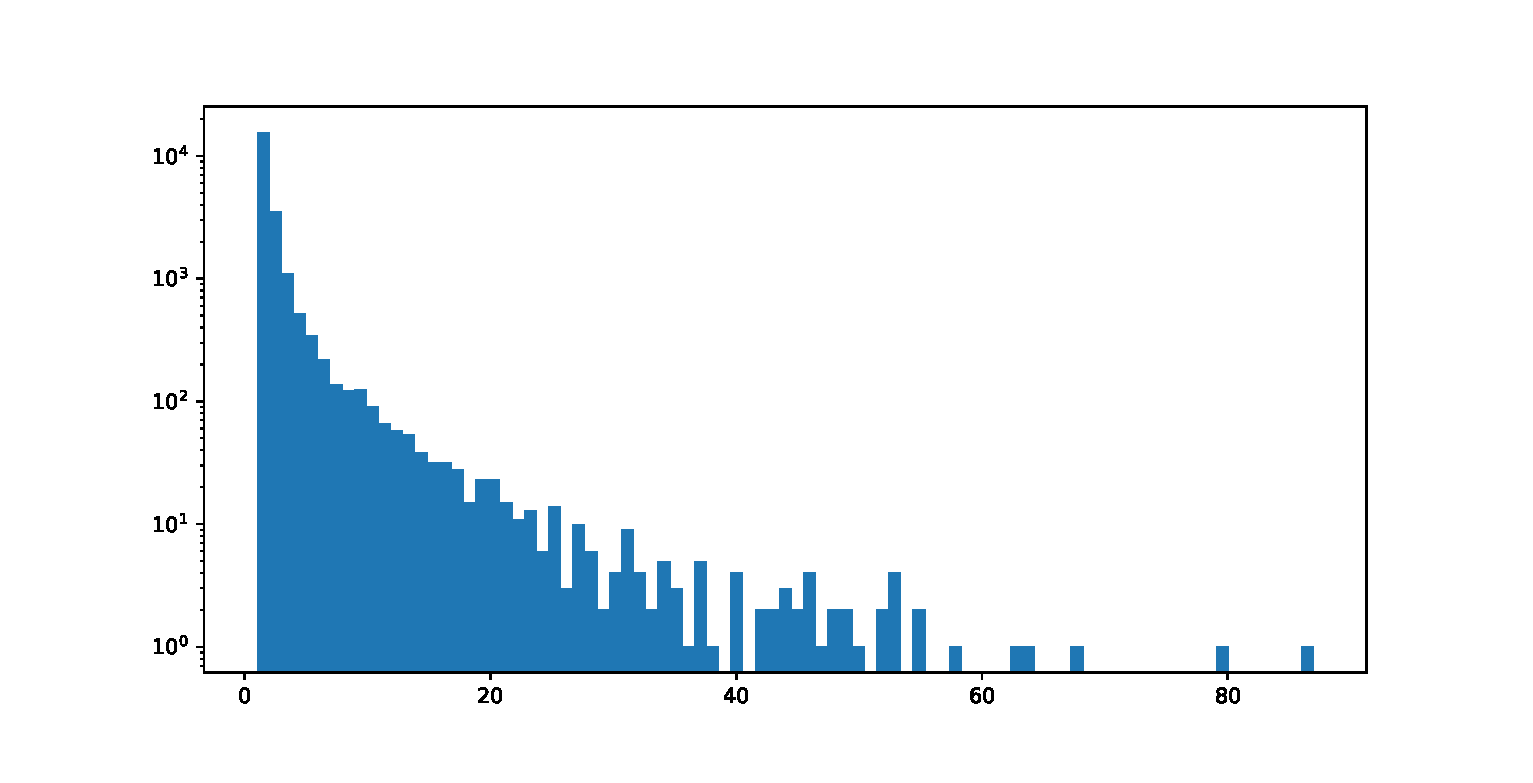
\includegraphics[width=.8\linewidth]{figures/cos02.eps}  
  \caption{cosine, 0.2}
  \label{fig:sub-cos02}
\end{subfigure}
\begin{subfigure}{.5\textwidth}
  \centering
  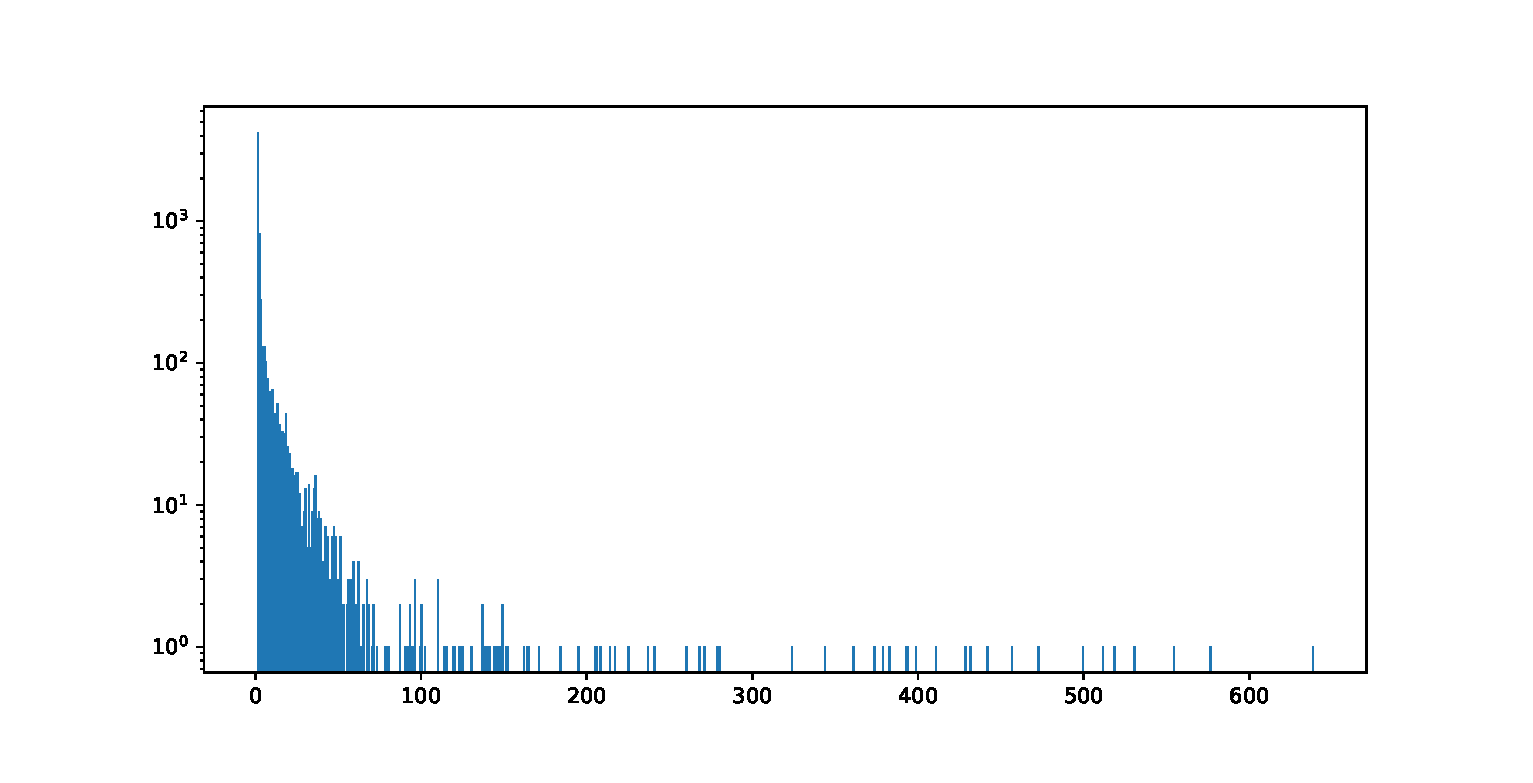
\includegraphics[width=.8\linewidth]{figures/softcos02.eps}  
  \caption{softcosine, 0.2}
  \label{fig:sub-softcos02}
\end{subfigure}

\begin{subfigure}{.5\textwidth}
  \centering
  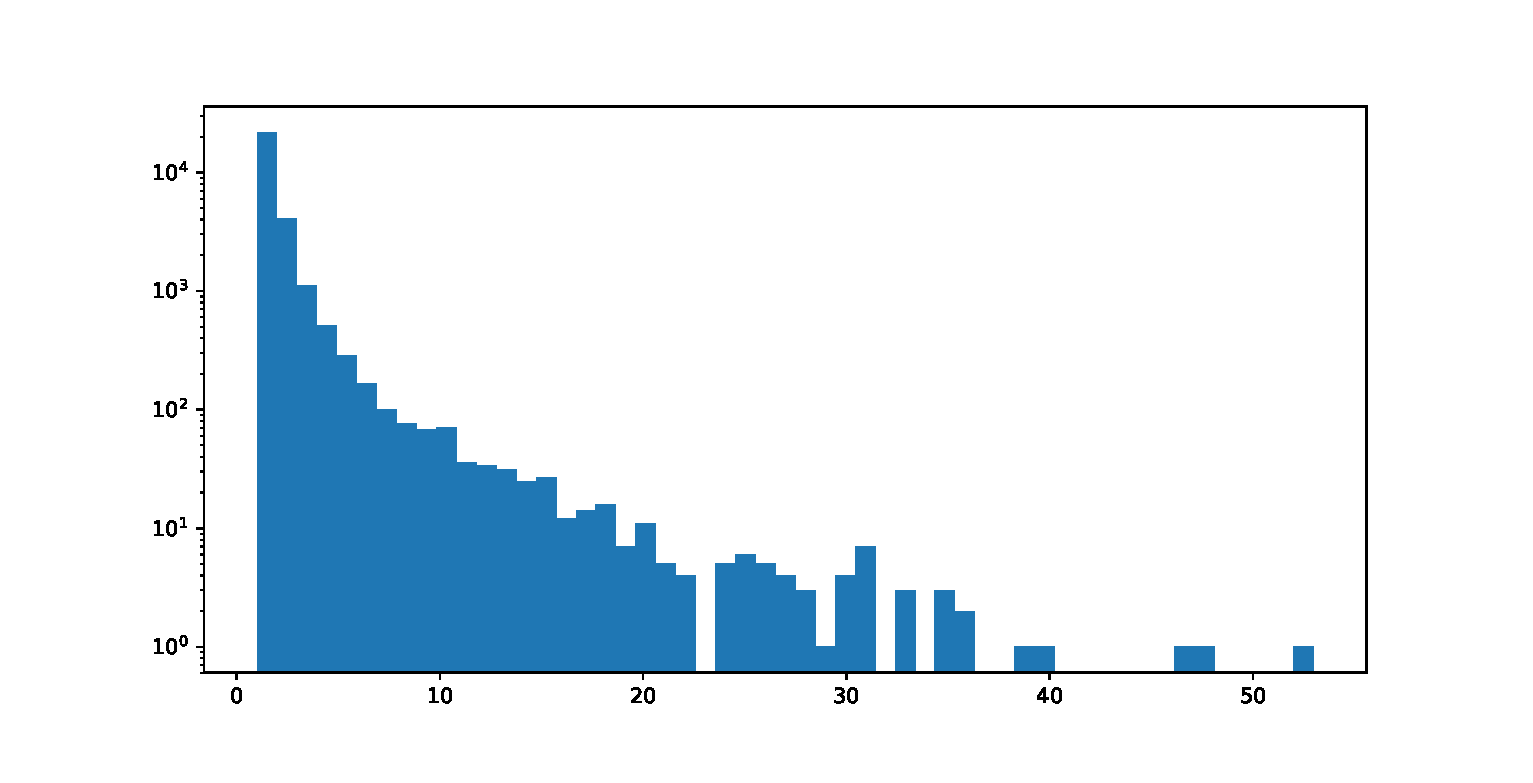
\includegraphics[width=.8\linewidth]{figures/cos03.eps}  
  \caption{cosine, 0.3}
  \label{fig:sub-cos03}
\end{subfigure}
\begin{subfigure}{.5\textwidth}
  \centering
  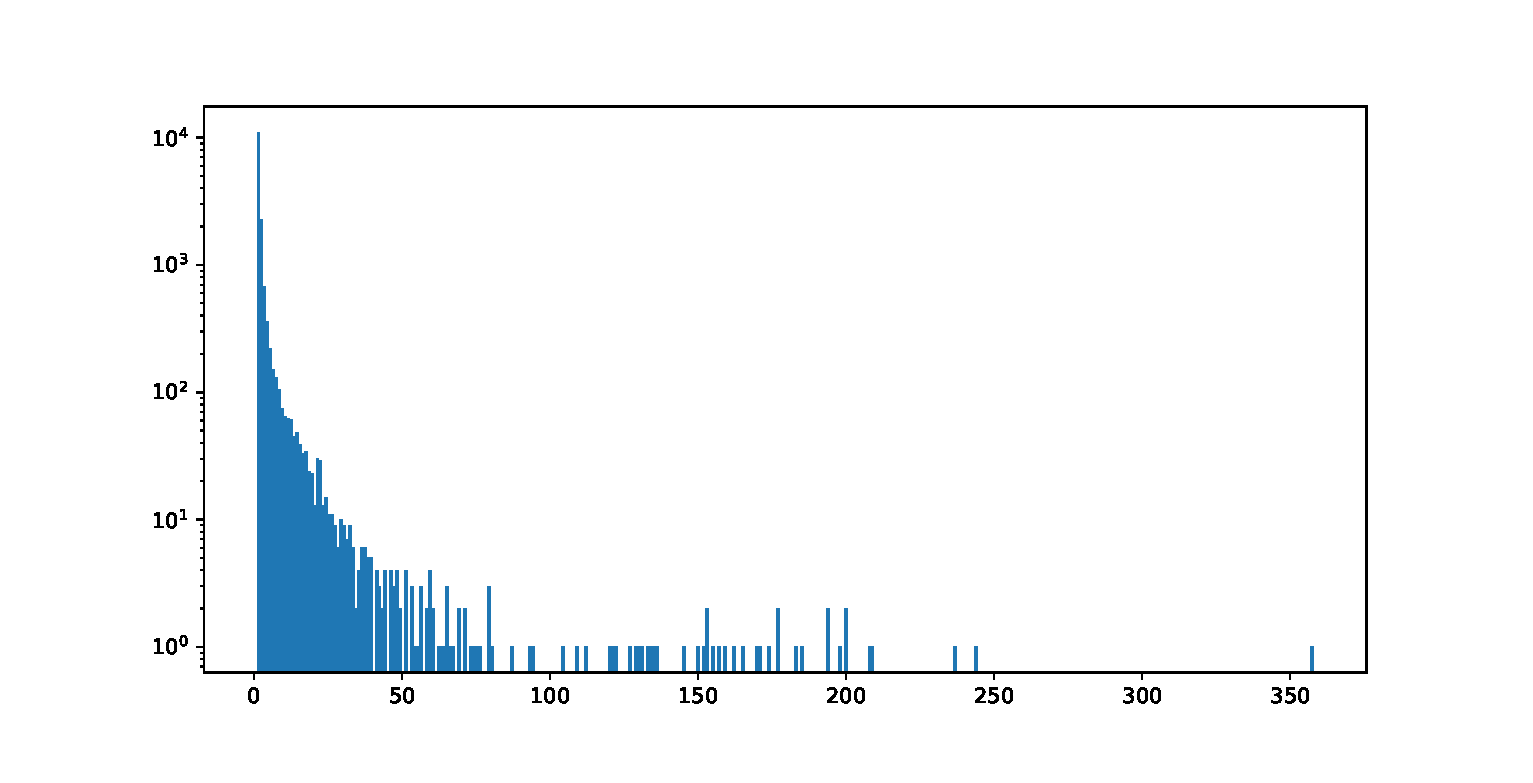
\includegraphics[width=.8\linewidth]{figures/softcos03.eps}  
  \caption{softcosine, 0.3}
  \label{fig:sub-softcos03}
\end{subfigure}

\begin{subfigure}{.5\textwidth}
  \centering
  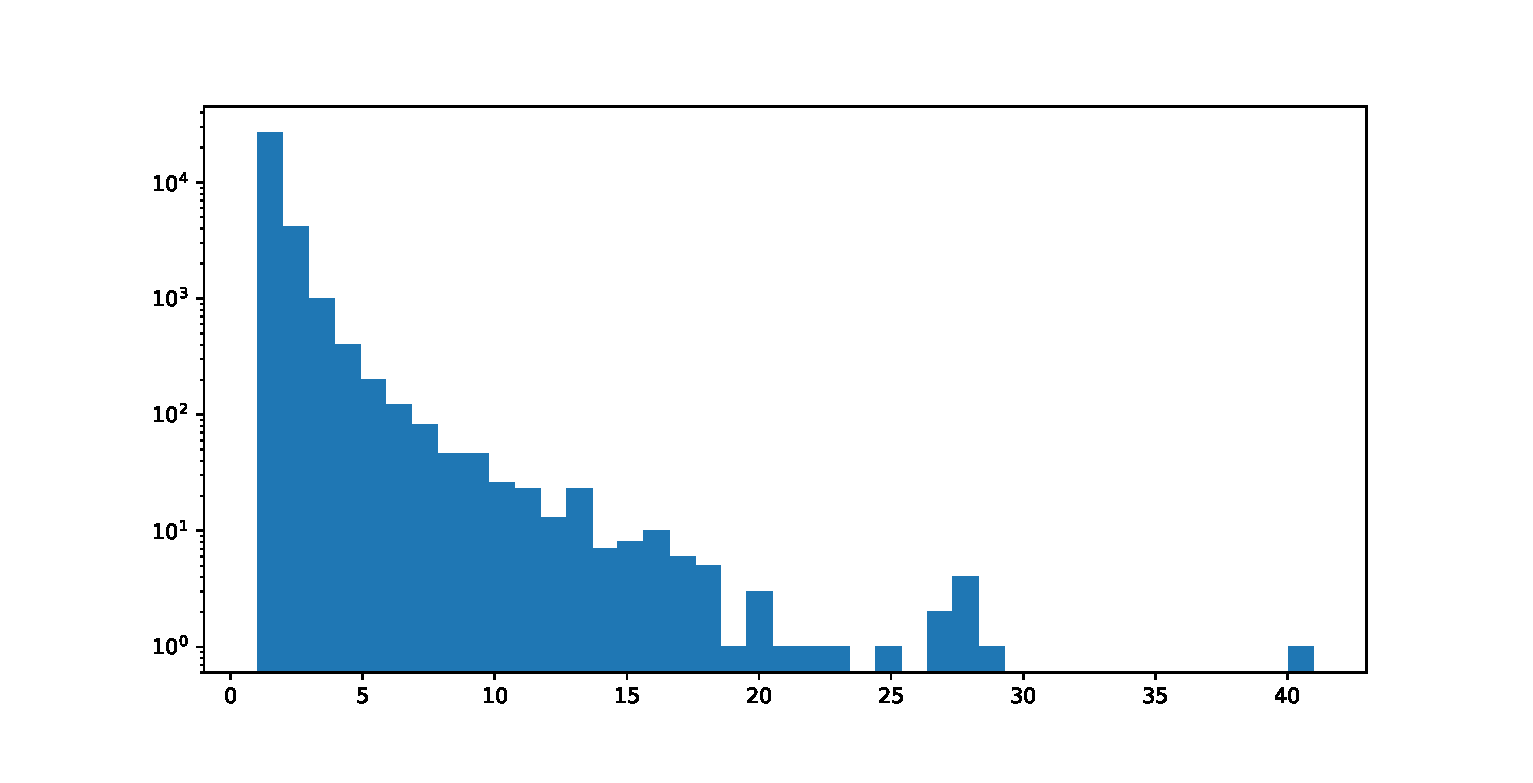
\includegraphics[width=.8\linewidth]{figures/cos04.eps}  
  \caption{cosine, 0.4}
  \label{fig:cos04}
\end{subfigure}
\begin{subfigure}{.5\textwidth}
  \centering
  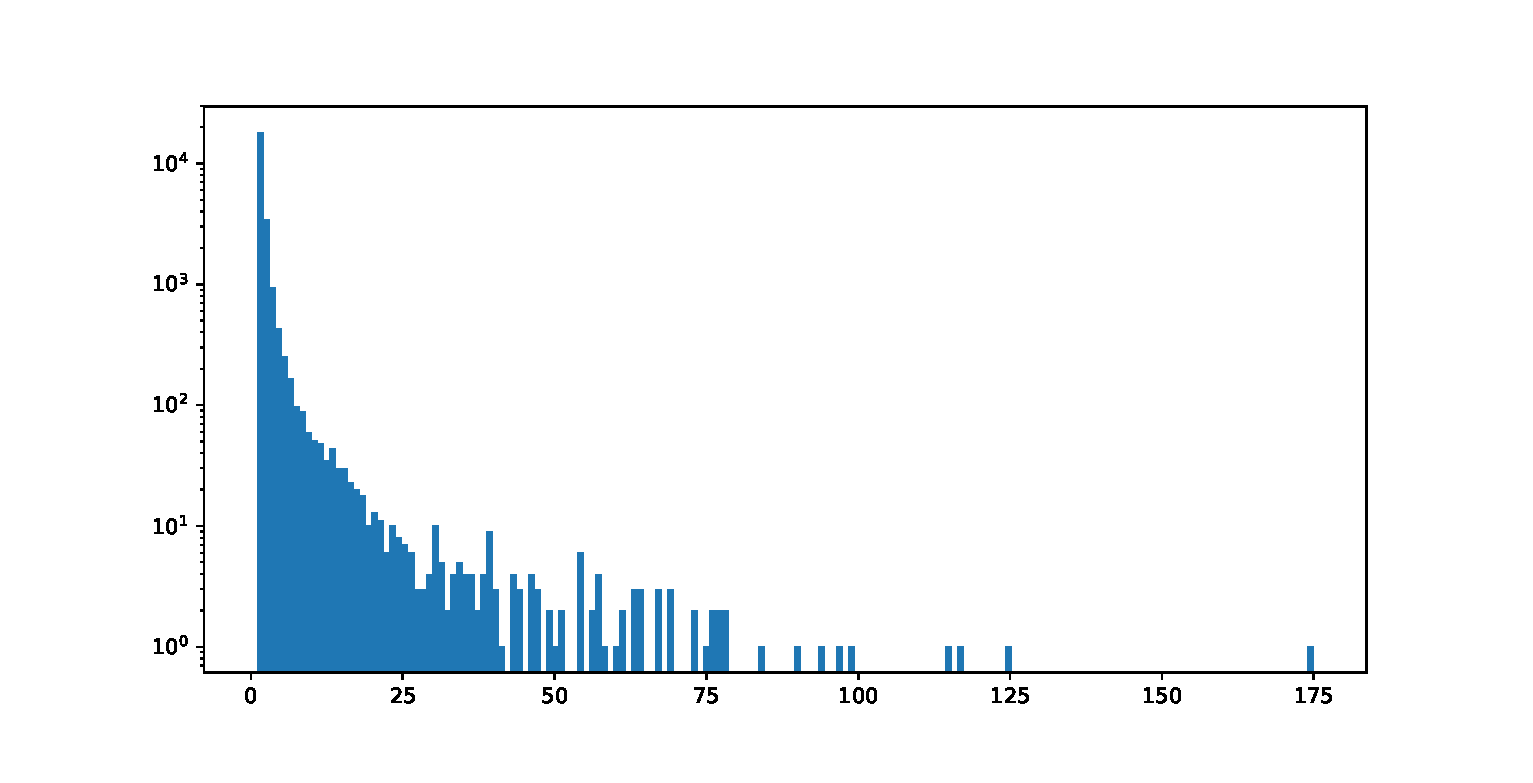
\includegraphics[width=.8\linewidth]{figures/softcos04.eps}  
  \caption{softcosine, 0.4}
  \label{fig:subsoftcos04}
\end{subfigure}

\begin{subfigure}{.5\textwidth}
  \centering
  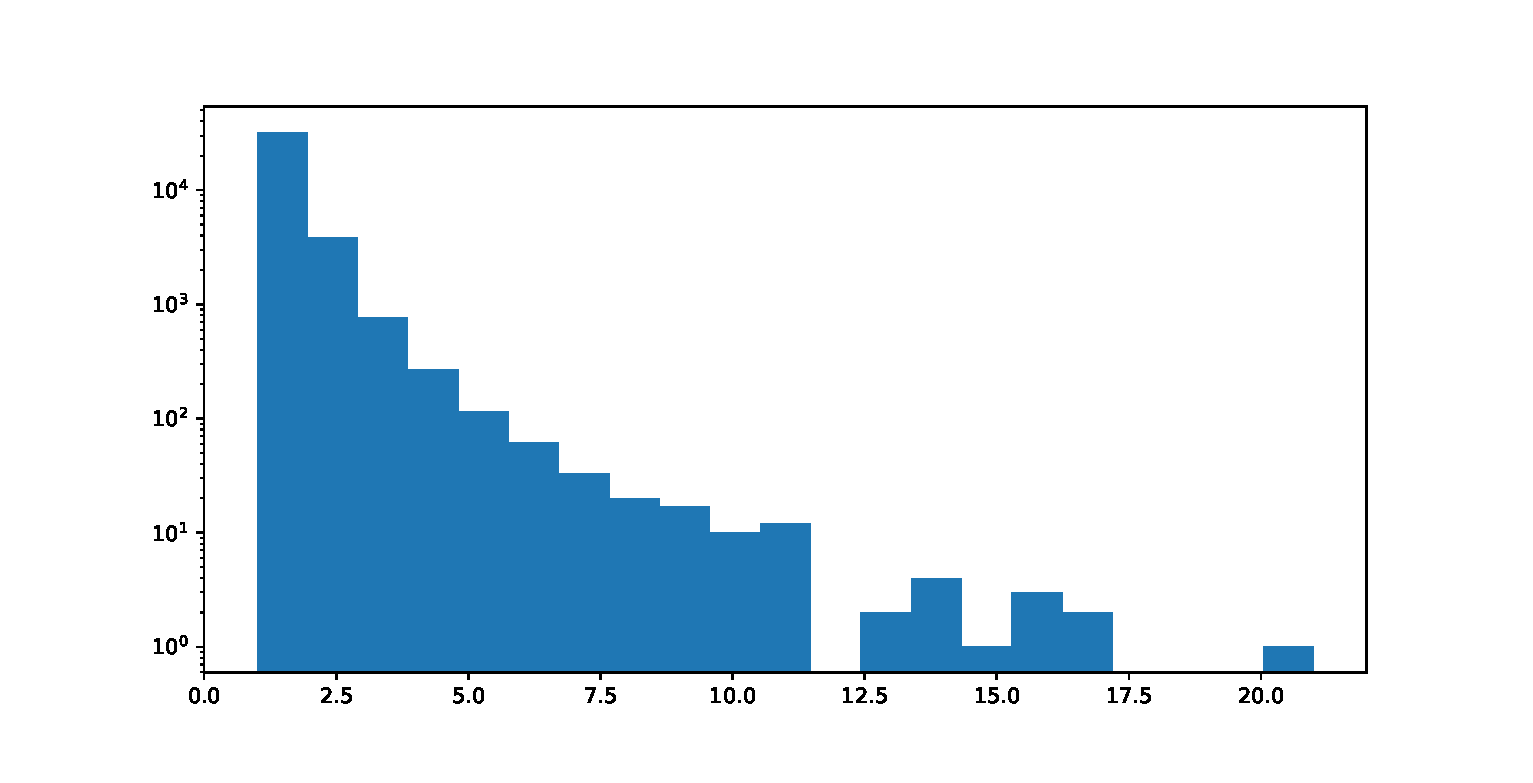
\includegraphics[width=.8\linewidth]{figures/cos05.eps}  
  \caption{cosine, 0.5}
  \label{fig:sub-cos05}
\end{subfigure}
\begin{subfigure}{.5\textwidth}
  \centering
  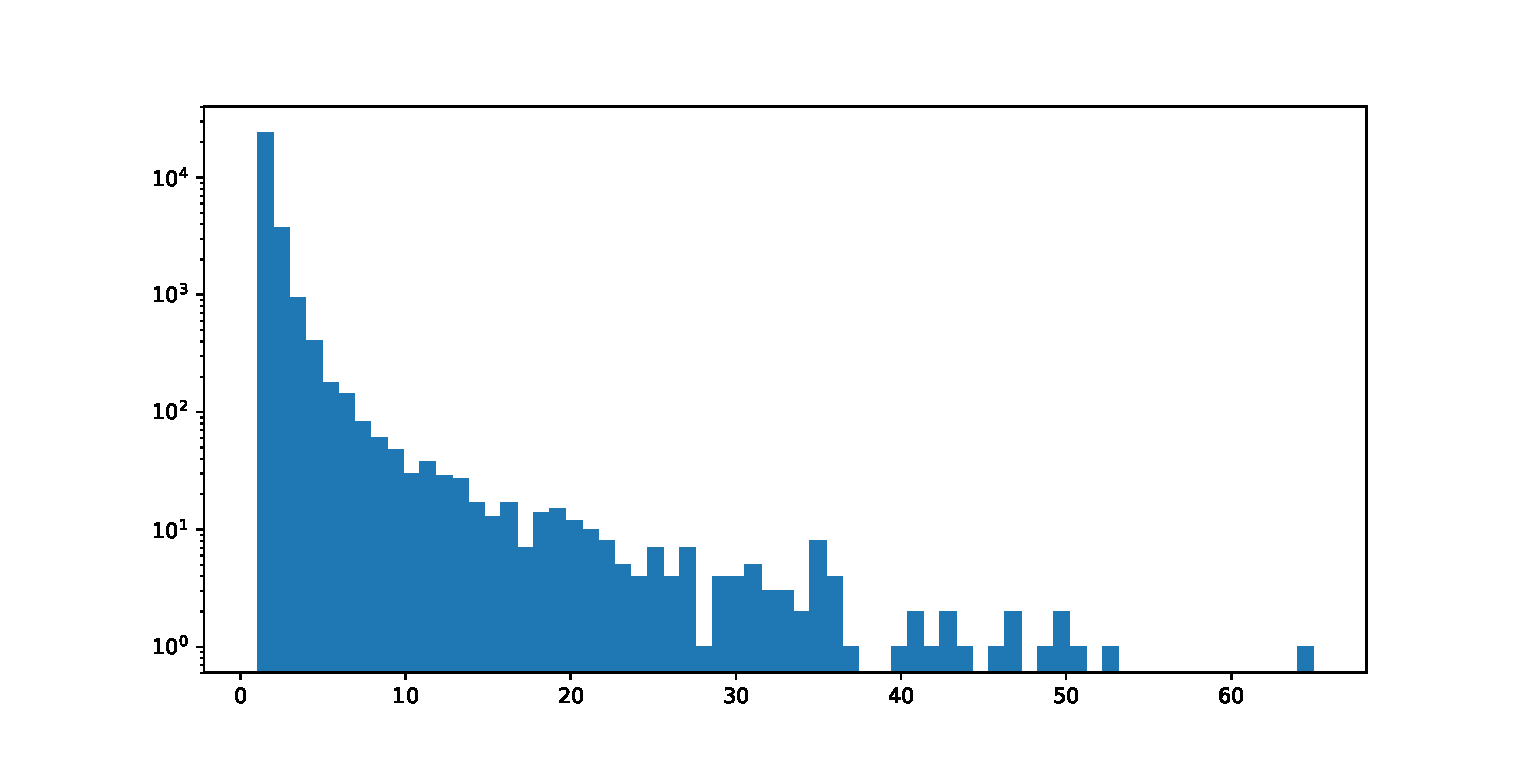
\includegraphics[width=.8\linewidth]{figures/softcos05.eps}  
  \caption{softcosine, 0.5}
  \label{fig:sub-softcos05}
\end{subfigure}

\begin{subfigure}{.5\textwidth}
  \centering
  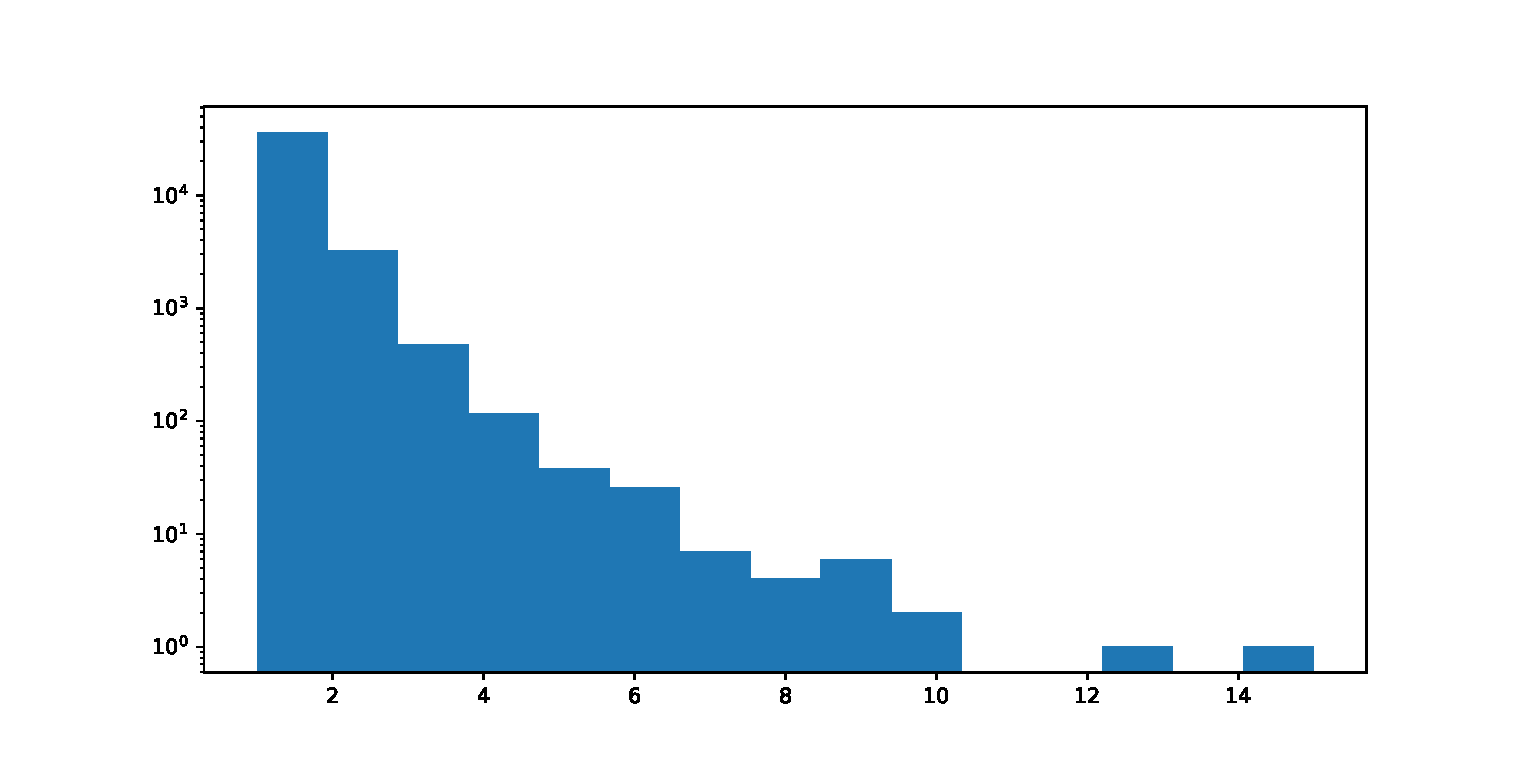
\includegraphics[width=.8\linewidth]{figures/cos06.eps}  
  \caption{cosine, 0.6}
  \label{fig:sub-cos06}
\end{subfigure}
\begin{subfigure}{.5\textwidth}
  \centering
  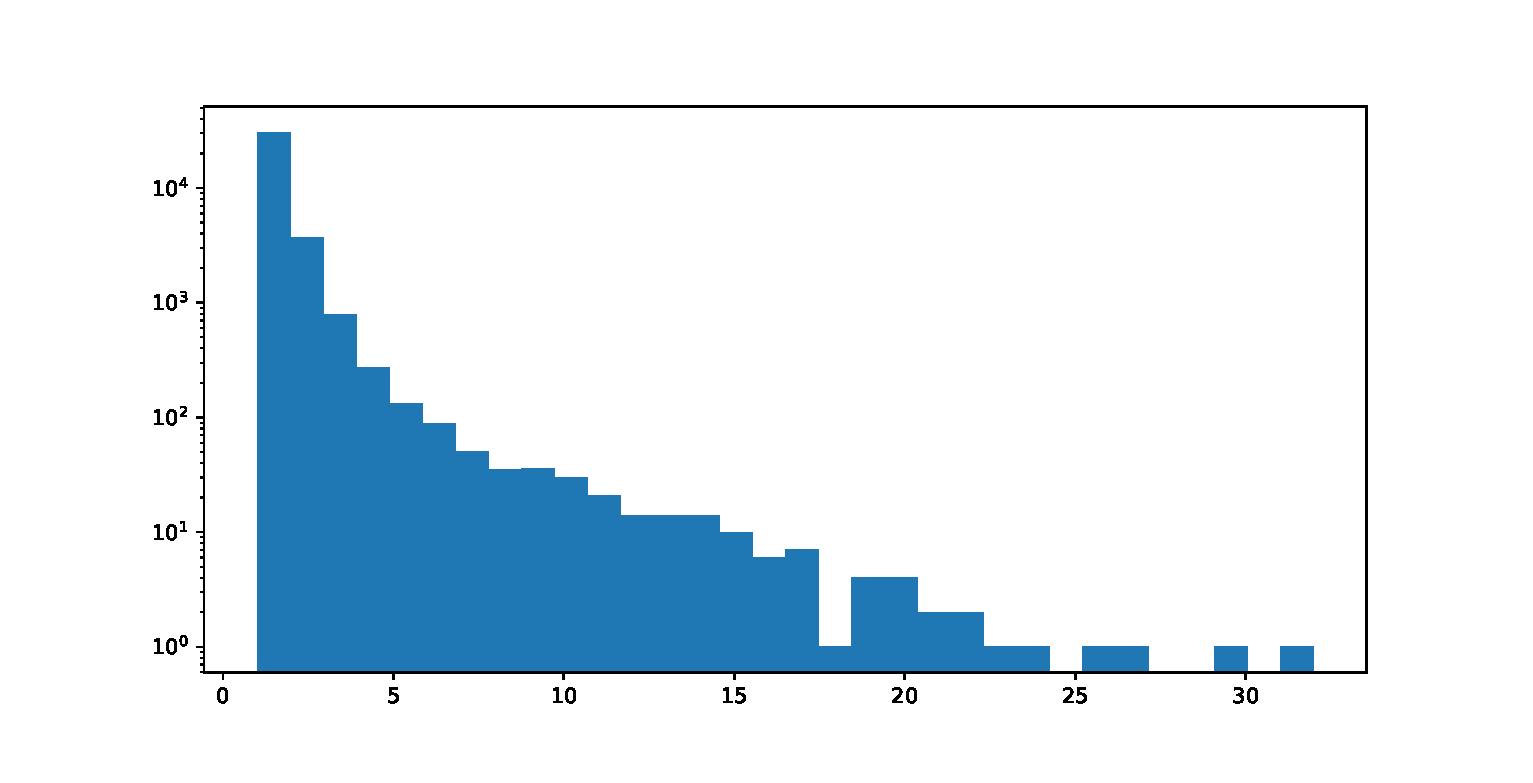
\includegraphics[width=.8\linewidth]{figures/softcos06.eps}  
  \caption{softcosine, 0.6}
  \label{fig:sub-softcos06}
\end{subfigure}
\caption{Histograms (logarithmic scale) of the number of articles per event using different similarity functions and thresholds.}
\label{fig:histograms}
\end{figure}

We therefore need to ask: Does the softcosine approach lead to a problematic false positive-rate?
The comparatively high maximum number of articles per event may suggest that. 
Yet, this is not the case: In the softcosine-0.6 model, the largest event consists of 35 articles. A manual inspection confirmed that all of them are related to a soccer match between Liverpool and Manchester. 
If we have a look at all events consisting of more than 20 articles, a similar picture arises. These 12 events span a diverse range of domains (sports, weather, an environmental disaster, \ldots), but only very few of these articles can be regarded as misclassified: in one of these 12 events, celebrity news are merged together with a sports event.

%Part of this is a question of selecting the right threshold (see next section).
%However, we also looked into the events that were




\section{Selecting a threshold}

Earlier work has suggested that similarity score of $>.2$ might cover the same topic \citep{Welbers2016}. However, as our experiments show, this threshold is too low to capture \emph{events} rather than broader issues or topics.

In fact, as we see in Table~\ref{tab:thresholds}, while a threshold of 0.2 may still work for a tf$\cdot$idf based cosine similarity score, it is clearly leading to too many false positives when employing soft cosine.
Out of 45k articles, only 4262 (thus, $<10\%$) were not assigned to an event, but the price we pay for this is too high: An event generating 551 articles is clearly implausible, and also mean and standard deviation seem too high, given that we study only three news sources (see also Figure~\ref{fig:histograms}).
A qualitative examination of a sample of detected events confirmed this.

More specifically, while there are some models and thresholds that are clearly inferior, there is not necessarily one ``best'' model.
In particular, we suggest that researchers make a well-informed tradeoff between more conservative models that offer a high precision (but miss some articles and some events) on the one hand and more encompassing models that recover more links articles and events at the expense of a slightly lower precision on the other hand.

\begin{table}[h]
\caption{Descriptives for different threshold/similarity combinations\label{tab:thresholds}}

\centering
\begin{tabular}{lrrrrrrrrrr}
\toprule
{} & \multicolumn{5}{c}{\textbf{cosine}} & \multicolumn{5}{c}{\textbf{softcosine}} \\
{} &    0.2  & 0.3 & 0.4 & 0.5 & 0.6 & 0.2 & 0.3  & 0.4 & 0.5 & 0.6  \\
\midrule
mean              &  2.03 & 1.58 & 1.35 & 1.21 & 1.12 & 6.78 & 2.89 & 1.88 & 1.51  & 1.27 \\
std              &  3.48 & 2.00 & 1.22 & 0.71 & 0.45  & 30.41 & 10.04 & 4.27 & 2.27 & 1.07 \\
max              &   88 & 53 & 41 & 21   & 15 & 551 & 367 & 161 & 70 & 30  \\
single-art.\\ events & 15626  & 21854  & 27135 & 32232 & 36348 & 4262 & 11043 & 18305 & 24337 & 30700 \\
multi-art.\\ events & 6685 & 6777 & 6241 & 5165 & 3899 & 2460 & 4736 & 5961 & 5940 & 5257 \\
\bottomrule
\end{tabular}
\end{table}


\begin{table}[h]
\begin{threeparttable}
\caption{Precision for different threshold/similarity combinations}
\label{tab:evaluation}

\centering
\begin{tabular}{lrrrr}
\toprule
\textbf{Similarity method}   & \textbf{Threshold} & \textbf{Prec. 1 (\%)} & \textbf{Prec. 2 (\%)} &\textbf{TP/max. TP}  \\
\midrule
cosine              & 0.4       & 74        & 88.52     & 223/268 \\
cosine              & 0.5       & 78        & 89.02     & 217/253 \\
cosine              & 0.6       & 89        & 94.39     & 204/225 \\
softcosine          & 0.4       & 56        & 76.20     & 234/521 \\
softcosine          & 0.5       & 65        & 81.77     & 236/379 \\
softcosine          & 0.6       & 75        & 86.92     & 222/289 \\
\bottomrule

\end{tabular}
%\begin{tablenotes}
\small
\textit{Note.} \textit{Precision 1:} The percentage of news events that are entirely clustered correctly. \textit{Precision 2:} The percentage of news articles that are correctly clustered. \textit{max. TP} is the number of articles that are assigned to an event in the sample; hence, the maximum number of true positives that can be achieved.
%\end{tablenotes}

\end{threeparttable}
\end{table}



\subsection{Answers to the research questions}
% RQ1 To what extent do the events covered overlap between outlets?
% RQ2 (a) Which kind of events enjoy the largest overlap, and (b) which kind of events are exclusive to specific outlets
% RQ3 How many articles do different outlets devote to the same event?


RQ1 asked to which extent the events overlap between outlets.
It seems to be surprising at first sight that the overlap is comparatively little (Figure~\ref{fig:venn}).
On closer inspection, though, this makes sense, as the answer to RQ2 shows.
RQ2 asked: (a) Which kind of events enjoy the largest overlap, and (b) which kind of events are exclusive to specific outlets?
To answer these questions, we compared the events that are covered by only one outlet with those that were covered by all.

\begin{figure}[h!]
%\captionsetup[subfigure]{justification=centering}
%\begin{subfigure}{.5\textwidth}
%  \centering
%  \includegraphics[width=.8\linewidth]{venn_softcos04.png}  
%  \caption{softcosine, 0.4}
%  \label{fig:sub-cos02}
%\end{subfigure}
%\begin{subfigure}{.5\textwidth}
  \centering
  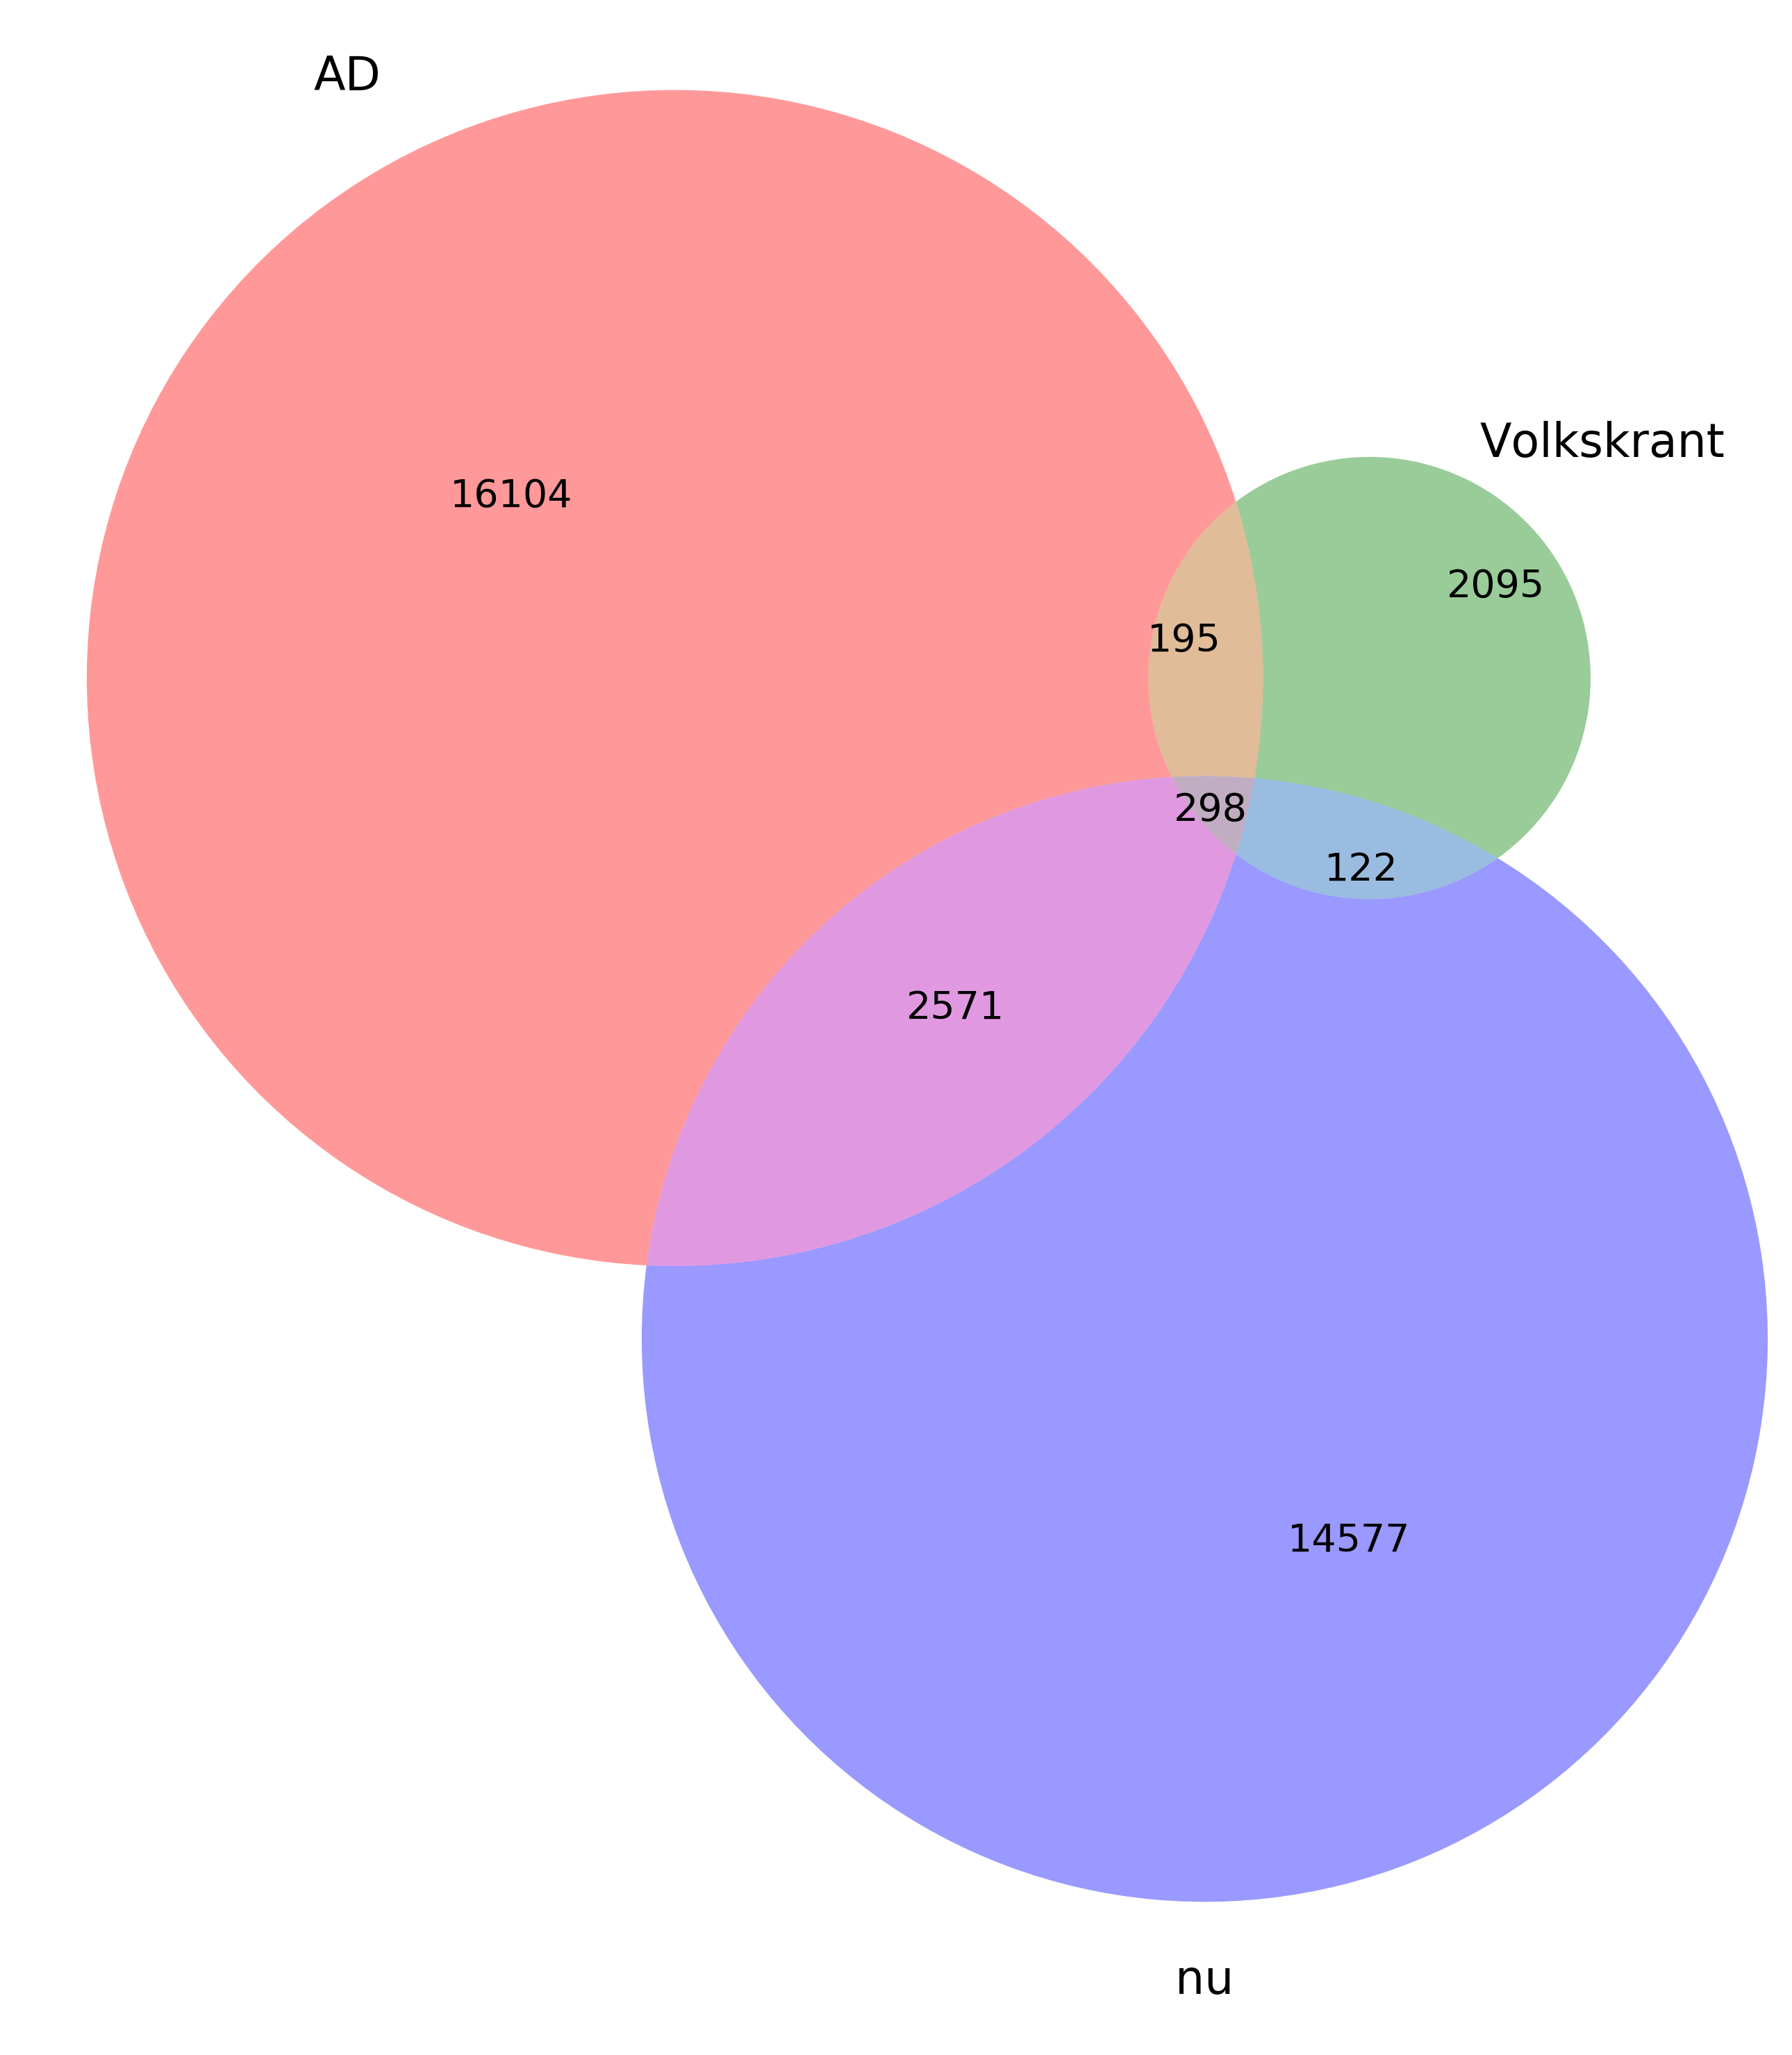
\includegraphics[width=.6\linewidth]{figures/vennsoft06.png}  
 % \caption{softcosine, 0.6}
  %\label{fig:sub-softcos02}
%\end{subfigure}
    \caption{Overlap in event coverage based on the the softcosine measure and a threshold of 0.6.}
    \label{fig:venn}
\end{figure}


For this, we decided to use the softcosine model with a threshold of 0.6. We chose for this model because it identifies more multiple-article events and misses less true positives than the standard cosine measure, even though this also came at the price of a lower but still very high precision, compared to the standard cosine models with a threshold of 0.5 or 0.6.
Others might want to make a different trade-off here.

First, we used a classifier that was pre-trained on Dutch news to classify our news events into four topics: Business, Politics, Entertainment and Other \citep{vermeer2018}. Figure \ref{fig:bar_topics} points out that AD and nu.nl are more likely to write about entertainment news events that other outlets do not cover.
In their exclusive news events, AD and nu.nl are relatively less likely to write about exclusive political events than Volkskrant (be it not in absolute numbers).
This very much fits what one would expect from these outlets, as Volkskrant is considered a quality newspaper, while AD is a popular newspaper with regional editions, and nu.nl an online-only outlet aiming at a very broad audience. 

\begin{figure}
    \centering
    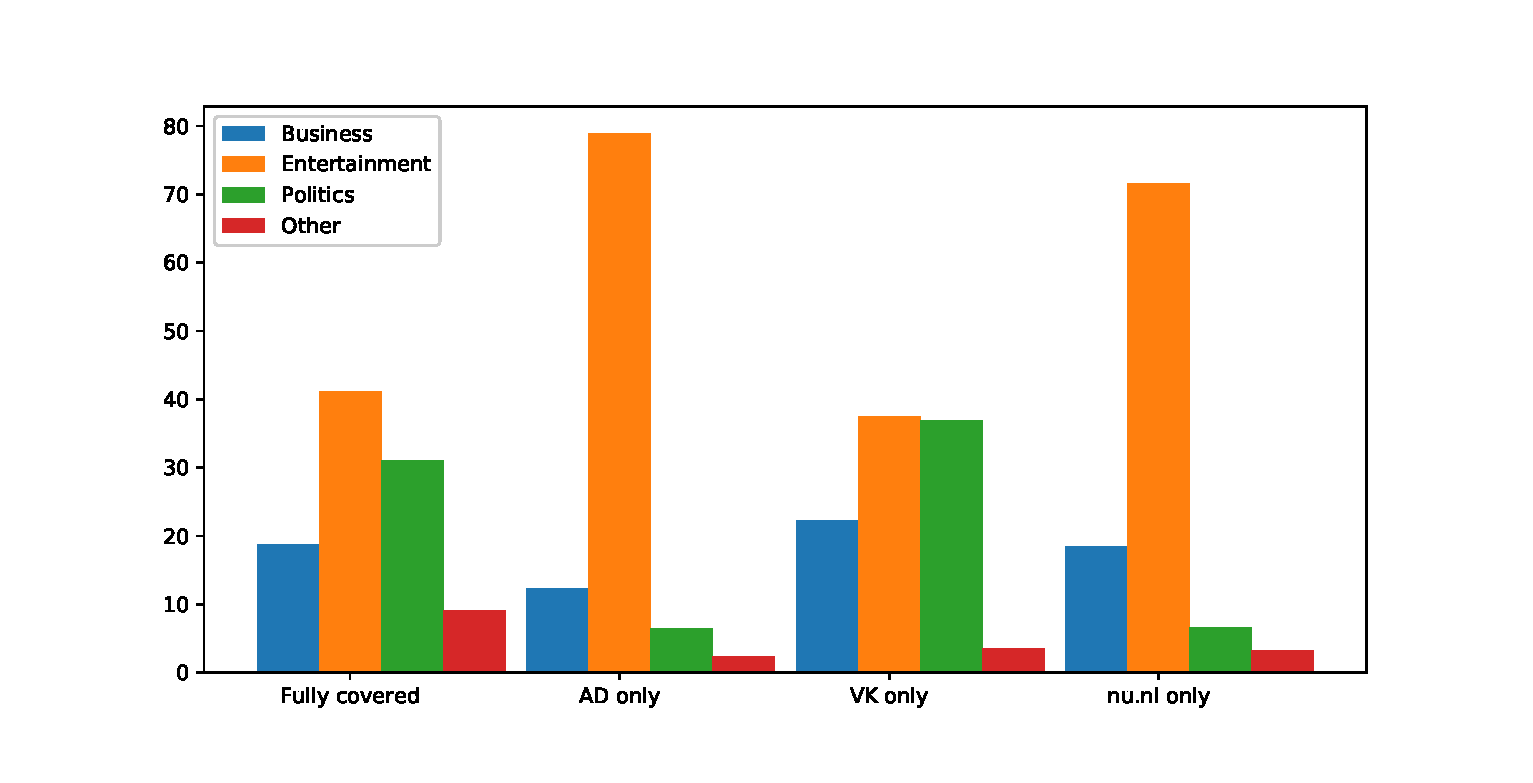
\includegraphics[width=\linewidth]{figures/classification.eps}
    \caption{Distribution of topics in fully covered, AD-only, Volkskrant-only and nu.nl-only news events}
    \label{fig:bar_topics}
\end{figure}

To confirm this picture in a more fine-grained way, we followed a suggestion by \citet{Rayson2000} and determined the most characteristic words for events covered by one outlet only versus fully-covered events by calculating their loglikelihood based on their observed and expected frequencies. 
In addition, and to ease interpretation, we did not only consider unigrams, but also bigrams.
Inspecting the 20 most characteristic words for each outlet, we see that most of these words are sport-related in the case of AD, entertainment and crime-related in the case of nu, and politics-related in the case of VK, even though the differences are less clear-cut for the last outlet (see Tables~\ref{tab:loglikelihood_ad}, \ref{tab:loglikelihood_vk}, and \ref{tab:loglikelihood_nu} in the Appendix).









\section{Conclusion and discussion}

Our aim in this paper was twofold: First, we offered a theoretical conceptualization of what we call a \emph{news event} and argued what this level of analysis can offer scholars of agenda setting, media hypes, and audience research.
Second, we explored computational approaches to detecting such events and to cluster articles accordingly. 

Regarding our first aim, we extended the literature by offering -- to the best of our knowledge -- the first attempt towards systematic definition of a news events v\`{i}s-a-v\`{i}s issues, topics, and story chains.
Regarding our second aim, we explored how these theoretical conceptualizations can be translated into a computational method to group news articles according to the events they cover even if the events are not known beforehand. 

In particular, we show that approaches based on literal overlap (such as the cosine similarity of tf$\cdot$idf representations) perform surprisingly well in our setup. 
However, they seem to be overly conservative and miss some articles that belong to an event, due to -- for instance -- differences in phrasing. 
Softcosine approaches can solve these issue due to the use of word embeddings. However, as we observed, this comes at a comparatively high cost by also merging articles that are about similar, but not identical events. 
Which approach is ultimately preferable may depend on the application.
We suggest that future research should tease out whether the strengths of both approaches can be combined. 

Regardless of whether one chooses the cosine or softcosine approach, our experiments demonstrate that these approaches work well and can be applied in a very efficient way by limiting the number of comparisons that need to be made.
Compared to a na\"ive compare-everything-with-everything approach, our approach based on a three-day-moving window is not only orders of magnitude faster, but renders the analysis of long-term datasets possible, as the number of comparisons only increases linearly instead of exponentially.
Next to these practical considerations, it leads to a lowers the amount of false positives as it prevents grouping articles about similar but temporally distinct events.


We by no means want to suggest that our approach is the only (or the best) way of automatically detecting news events.
We have shown that the combination of the Leiden network clustering algorithm with cosine (or softcosine) based similarity metrics, applied to a moving-window of news articles, can be a feasible approach.
We suggest, though, further explore alternatives and to systematically compare them.

In order to do so, though, we need to systematically think about the right metrics for doing so.
For instance, given that the population of all events is assumed to be unknown, as are the number of articles per event, we can calculate a measure of precision by checking how many of the articles ascribed to an event indeed are about the event; but we cannot calculate a measure of recall that tells us whether we found all articles about the event, or whether we indeed found all events.

Some \citep{Welbers2016,Nicholls2018} have approached the issue by randomly drawing pairs of articles, checking manually whether they are about the same event, and then comparing their assessment with the grouping their model produced. While this approach does allow the calculation of both precision and recall, it requires a lot of pairs to be evaluated (as most randomly drawn pairs will not be about the same event) and -- in our view -- in fact answers a different question then the questions that should be of core interest to the evaluation: (1) How many articles ascribed to an event indeed belong to it?; (2) How many articles were not assigned to any event though they in fact do belong to one?; and (3) How many events did we miss?
Future research needs to assess what the best feasible evaluation criteria for news event detection are.

We finally demonstrated how our method can be used in a small case study. This suggested that overlap between different online news outlets might actually be rather low if it comes to the specific events covered, and probably lower than an analysis on the issue or topic level would suggest. Yet, the differences made immediately sense once we looked in more detail into which events differed in their coverage: Both a top-down topic classification as a bottom-up inspection of most over-represented uni- and bigrams showed that the quality paper covered political events that the other outlets missed, the popular newspaper covered additional sports events, and the online-only news site offered crime and entertainment events that the other outlets did not cover.

The conceptual and methodological considerations in this paper as well as these first applications to a news dataset should, however, rather be seen as the beginning than as the end: as the beginning towards the development of a robust and easy-to-use method to detect news events. In the end, this will greatly improve the way how we can make sense of media content, but also of media use data.



%More applications:
%In future work, we could even re-use the same approach to study news diets of individual users if we have access to, for instance, their browsing history. We could then determine in how far people ``miss out'' on events, and in how far there is a hard core of events everyone is aware of and how this core looks like.


%Refinement of method:
%...
% ....




\bibliography{references}

\clearpage

\section{Appendix}

\setcounter{figure}{0}
\renewcommand{\thefigure}{A\arabic{figure}}


\setcounter{table}{0}
\renewcommand{\thetable}{A\arabic{table}}




\begin{figure}[h!]
\captionsetup[subfigure]{justification=centering}
\begin{subfigure}{.5\textwidth}
  \centering
  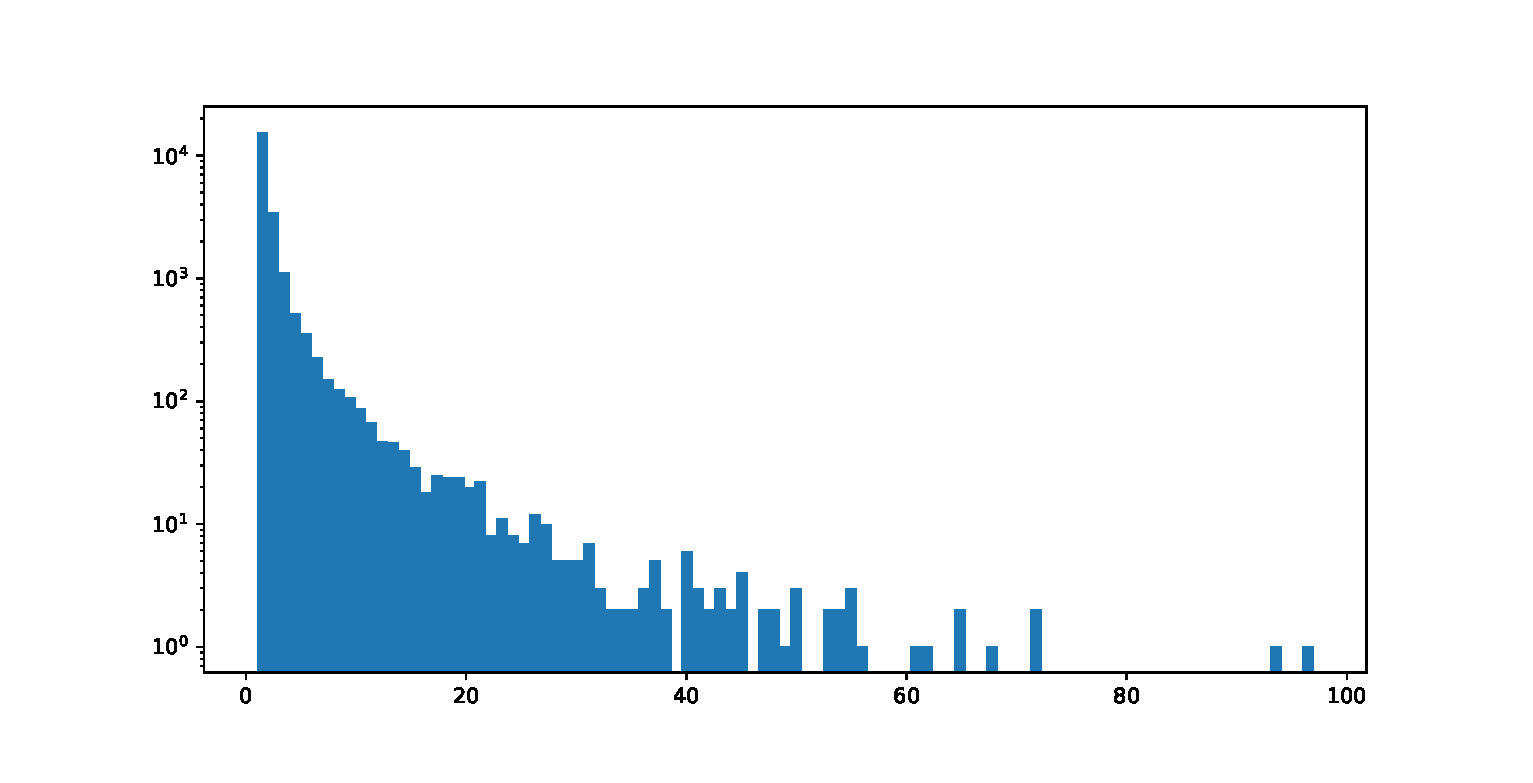
\includegraphics[width=.8\linewidth]{figures/infomapcos02.eps}  
  \caption{cosine, 0.2}
  \label{fig:sub-infomapcos02}
\end{subfigure}
\begin{subfigure}{.5\textwidth}
  \centering
  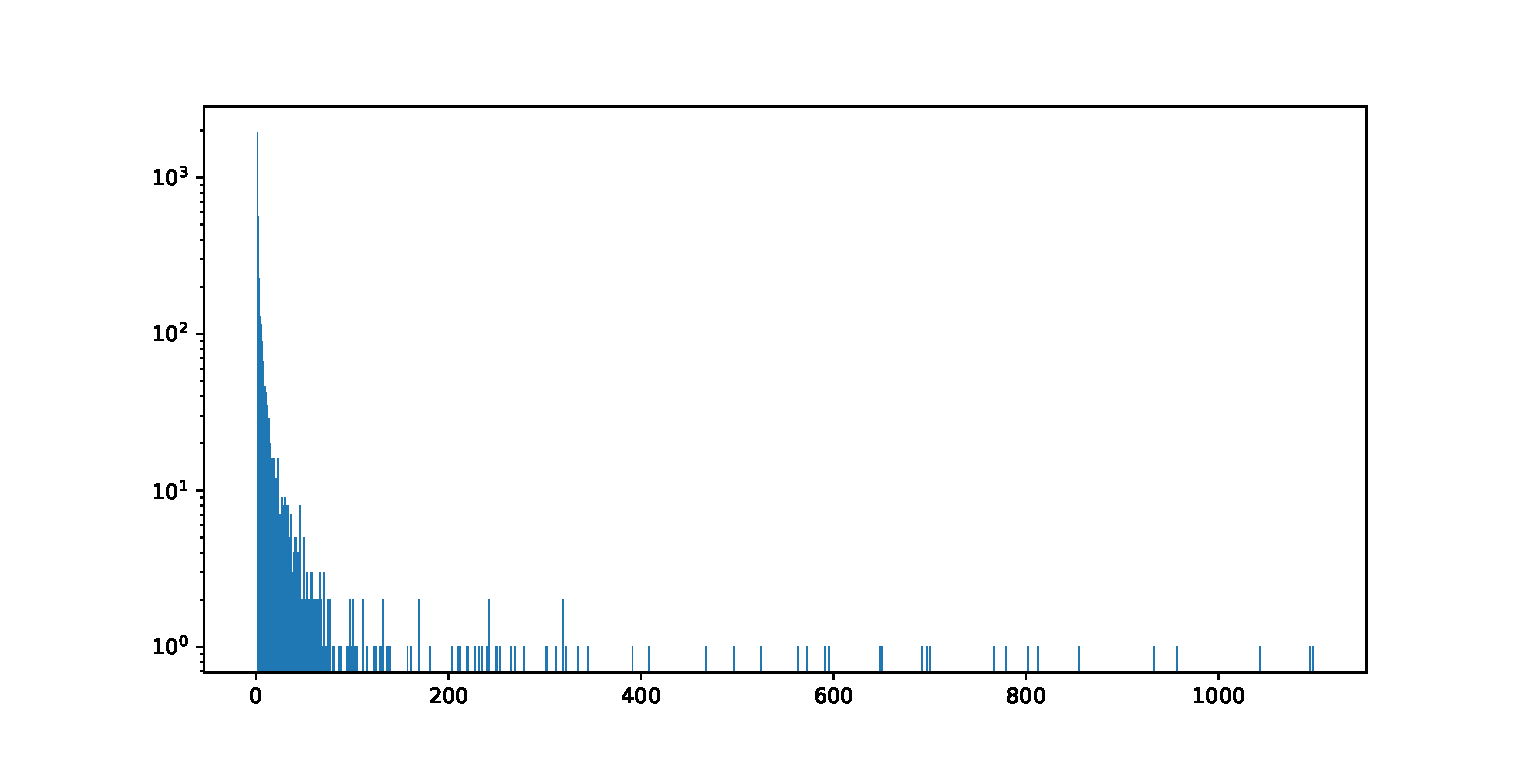
\includegraphics[width=.8\linewidth]{figures/infomapsoft02.eps}  
  \caption{softcosine, 0.2}
  \label{fig:sub-infomapsoftcos02}
\end{subfigure}

\begin{subfigure}{.5\textwidth}
  \centering
  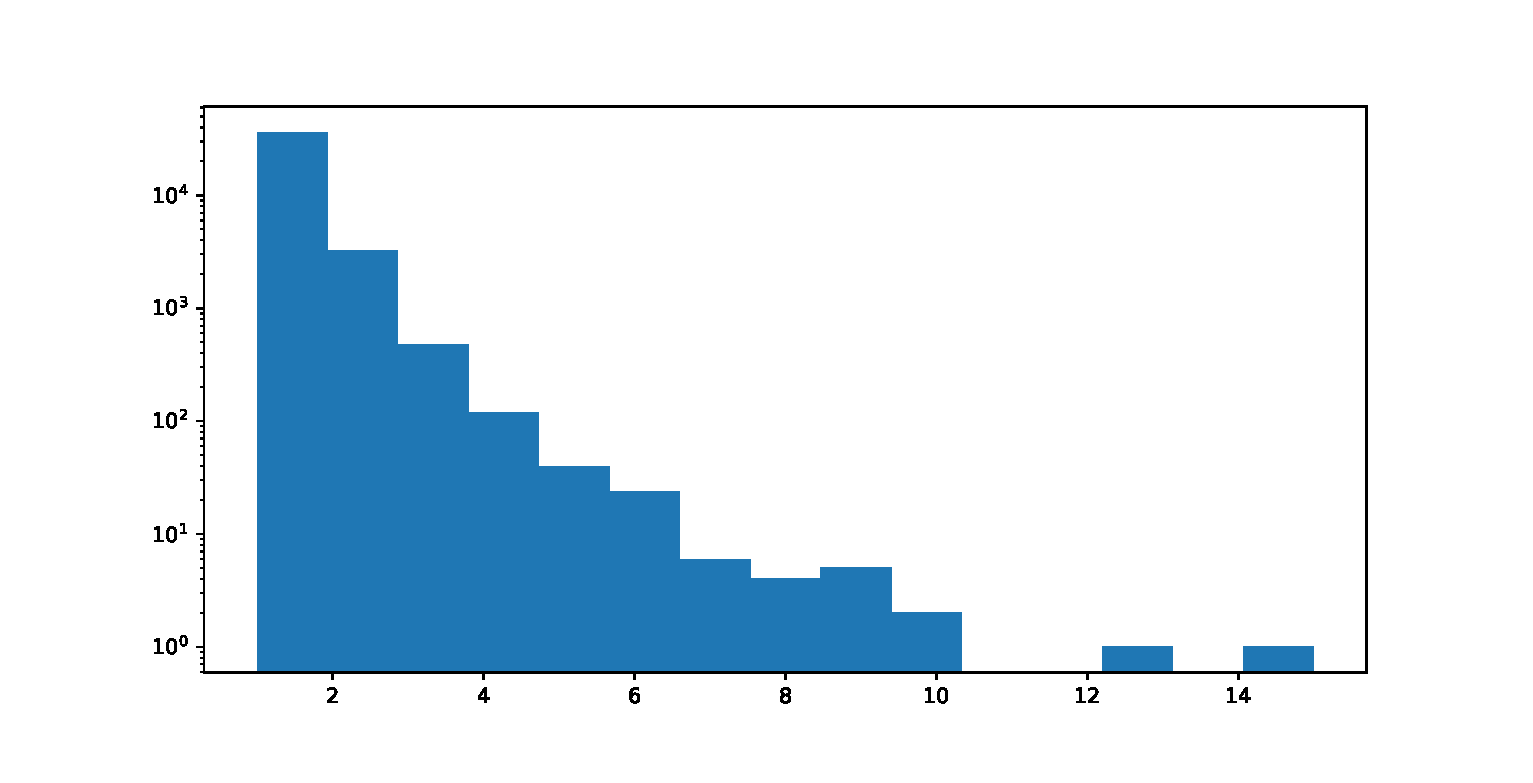
\includegraphics[width=.8\linewidth]{figures/infomapcos06.eps}  
  \caption{cosine, 0.6}
  \label{fig:sub-infomapcos02}
\end{subfigure}
\begin{subfigure}{.5\textwidth}
  \centering
  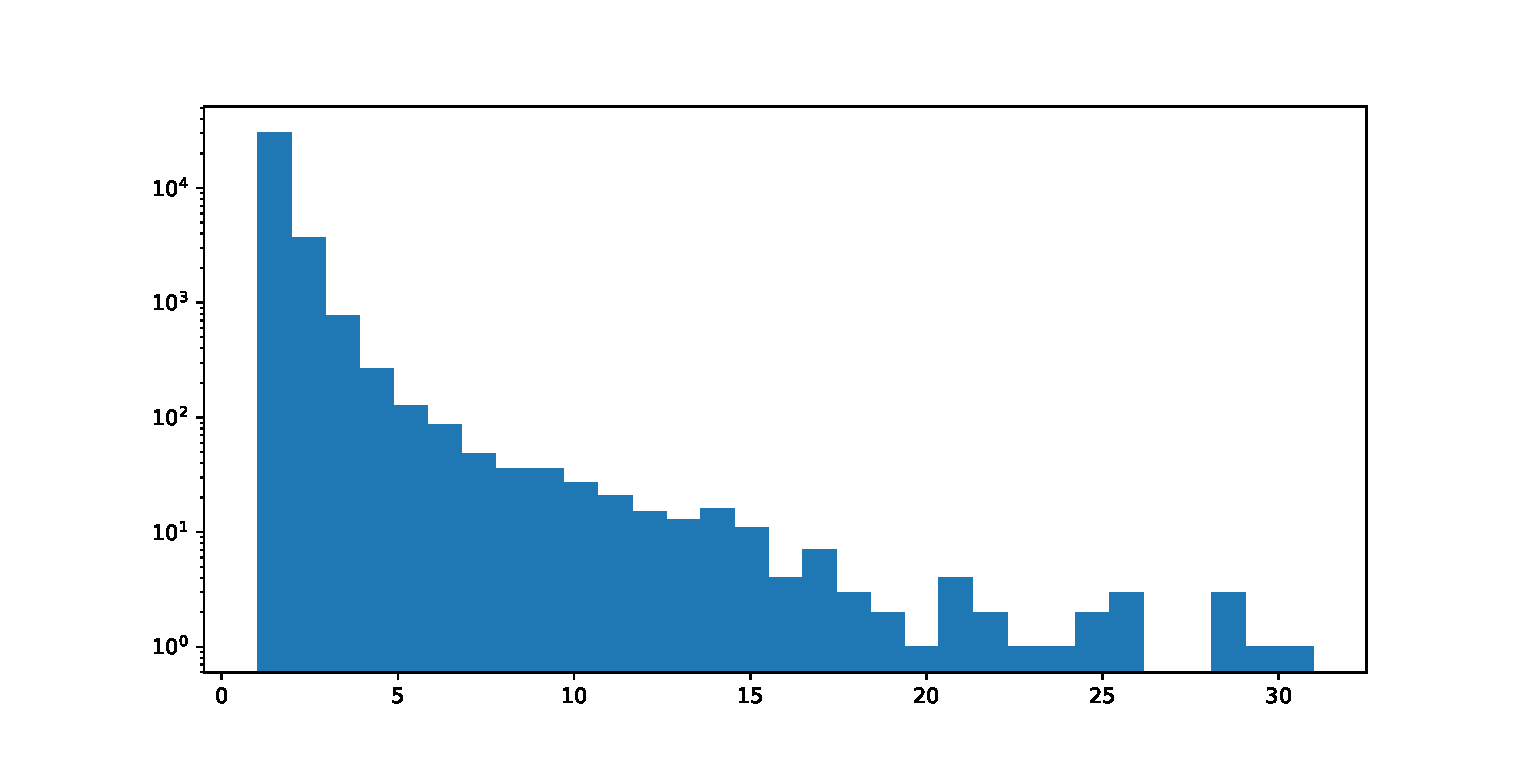
\includegraphics[width=.8\linewidth]{figures/infomapsoft06.eps}  
  \caption{softcosine, 0.6}
  \label{fig:sub-infomapsoftcos02}
\end{subfigure}
\caption{Histograms (logarithmic scale) of the number of articles per event using different similarity functions and thresholds when using Infomap partitioning}
\label{fig:infomap}
\end{figure}



\begin{table}[h]
\caption{Descriptives for different threshold/similarity combinations when using Infomap partitioning\label{tab:thresholds_infomap}}

\centering
\begin{tabular}{lrrrr}
\toprule
{} & \multicolumn{2}{c}{\textbf{cosine}} & \multicolumn{2}{c}{\textbf{softcosine}} \\
{} &    0.2 & 0.6 & 0.2 & 0.6 \\
\midrule
mean                 & 2.04   &  1.12  &  12.14  &  1.12\\
std                  &  3.64  &  0.48  &  63.96  &  0.48\\
max                  &  97    &  15    &  1099   &  15\\
single-art.events &  15529 &  3647  &  1951   &  3647\\
multi-art. events  &  6628  &  3902  &  1805   &  3902\\
\bottomrule
\end{tabular}
\end{table}


\begin{table}[h]
\caption{Most characteristic words for AD-only events (compared to fully-covered events)}
\label{tab:loglikelihood_ad}
\begin{tabular}{rlrrrr}
\toprule
loglikelihood & word & \multicolumn{2}{c}{AD} & \multicolumn{2}{c}{Fully} \\
{} &         {}  & observed &  expected & observed  &  expected  \\
\midrule
    102.042086 &      seizoen &              2048 &            1981.63 &                 7 &              73.37 \\
     65.001496 &         auto &              2045 &            1988.38 &                17 &              73.62 \\
     64.408414 &       finale &              1012 &             976.83 &                 1 &              36.17 \\
     61.066777 &    wedstrijd &              1349 &            1306.62 &                 6 &              48.38 \\
     57.723314 &       punten &              1421 &            1377.98 &                 8 &              51.02 \\
     55.118750 &         ajax &              1049 &            1014.44 &                 3 &              37.56 \\
     53.186585 &         club &              1462 &            1419.45 &                10 &              52.55 \\
     45.697166 &           fc &               977 &             945.98 &                 4 &              35.02 \\
     45.606776 &           wk &               745 &             719.37 &                 1 &              26.63 \\
     44.665614 &        ploeg &               961 &             930.55 &                 4 &              34.45 \\
     43.780026 &          won &              1133 &            1099.30 &                 7 &              40.70 \\
     42.668881 &  dit\_seizoen &               703 &             678.87 &                 1 &              25.13 \\
     41.808926 &    de\_finale &               575 &             554.47 &                 0 &              20.53 \\
     38.900479 &         real &               535 &             515.90 &                 0 &              19.10 \\
     38.239477 &       league &              1203 &            1169.69 &                10 &              43.31 \\
     37.796480 &      trainer &               715 &             691.40 &                 2 &              25.60 \\
     36.861917 &        beste &              1657 &            1617.13 &                20 &              59.87 \\
     36.646432 &       oranje &               504 &             486.01 &                 0 &              17.99 \\
     36.499073 &        meter &              1011 &             981.65 &                 7 &              36.35 \\
     36.355588 &          psv &               500 &             482.15 &                 0 &              17.85 \\
\bottomrule
\end{tabular}

\end{table}

\begin{table}[]
\caption{Most characteristic words for VK-only events  (compared to fully-covered events)}
\label{tab:loglikelihood_vk}
\begin{tabular}{rlrrrr}
\toprule
loglikelihood & word & \multicolumn{2}{c}{Volkskrant} & \multicolumn{2}{c}{Fully} \\
{} &         {}  & observed &  expected & observed  &  expected  \\
\midrule
     28.980838 &               project &               170 &             156.11 &                 0 &              13.89 \\
     28.682444 &                  zegt &              3852 &            3762.25 &               245 &             334.75 \\
     27.194927 &                   may &               338 &             315.89 &                 6 &              28.11 \\
     25.040629 &                brexit &               344 &             322.32 &                 7 &              28.68 \\
     23.790320 &                  gele &               214 &             198.35 &                 2 &              17.65 \\
     23.300058 &               vrouwen &               728 &             695.15 &                29 &              61.85 \\
     21.327260 &             politieke &               911 &             875.13 &                42 &              77.87 \\
     21.309440 &                bouwen &               125 &             114.79 &                 0 &              10.21 \\
     20.116111 &              dan\_hier &               118 &             108.36 &                 0 &               9.64 \\
     19.604685 &  volkskrant\_politiek’ &               115 &             105.60 &                 0 &               9.40 \\
     19.569623 &              europese &              1083 &            1045.02 &                55 &              92.98 \\
     19.434209 &       hier\_volkskrant &               114 &             104.69 &                 0 &               9.31 \\
     18.752307 &         ontvangenvink &               110 &             101.01 &                 0 &               8.99 \\
     18.752307 &   email\_ontvangenvink &               110 &             101.01 &                 0 &               8.99 \\
     18.752307 &     ontvangenvink\_dan &               110 &             101.01 &                 0 &               8.99 \\
     18.651879 &             patiënten &               273 &             256.20 &                 6 &              22.80 \\
     18.581832 &          elke\_werkdag &               109 &             100.09 &                 0 &               8.91 \\
     18.355639 &          de\_politieke &               227 &             212.13 &                 4 &              18.87 \\
     18.240880 &      nieuwsbrief\_elke &               107 &              98.26 &                 0 &               8.74 \\
     18.238464 &                hesjes &               148 &             136.83 &                 1 &              12.17 \\
\bottomrule
\end{tabular}
\end{table}
\begin{table}
\caption{Most characteristic words for nu.nl-only events (compared to fully-covered events)}
\label{tab:loglikelihood_nu}
\begin{tabular}{rlrrrr}
\toprule
loglikelihood & word & \multicolumn{2}{c}{nu.nl} & \multicolumn{2}{c}{Fully} \\
{} &         {}  & observed &  expected & observed  &  expected  \\
\midrule
    139.205076 &            uur &              4749 &            4612.88 &                55 &             191.12 \\
     99.492133 &        seizoen &              1799 &            1734.15 &                 7 &              71.85 \\
     97.931920 &        politie &              5605 &            5475.15 &                97 &             226.85 \\
     80.452705 &            the &              2447 &            2373.66 &                25 &              98.34 \\
     79.508001 &           auto &              2058 &            1992.45 &                17 &              82.55 \\
     71.571045 &     de\_politie &              4352 &            4253.76 &                78 &             176.24 \\
     70.932496 &           film &              1518 &            1466.25 &                 9 &              60.75 \\
     70.314206 &           nunl &              1396 &            1347.18 &                 7 &              55.82 \\
     69.152095 &          meldt &              2215 &            2149.92 &                24 &              89.08 \\
     62.732081 &         uur\_op &               885 &             850.75 &                 1 &              35.25 \\
     60.881861 &    aangehouden &              1318 &            1273.25 &                 8 &              52.75 \\
     60.201501 &           ajax &              1007 &             969.82 &                 3 &              40.18 \\
     58.331796 &      programma &              1437 &            1390.39 &                11 &              57.61 \\
     57.626913 &           2019 &              1216 &            1174.34 &                 7 &              48.66 \\
     57.195878 &            man &              3714 &            3632.50 &                69 &             150.50 \\
     56.835079 &       festival &               700 &             672.15 &                 0 &              27.85 \\
     55.548227 &  politie\_heeft &               945 &             910.29 &                 3 &              37.71 \\
     54.080711 &       meldt\_de &               855 &             822.91 &                 2 &              34.09 \\
     53.673115 &          autos &               770 &             740.33 &                 1 &              30.67 \\
     52.780669 &          serie &               838 &             806.58 &                 2 &              33.42 \\

\bottomrule
\end{tabular}
\end{table}


\end{document}

